\documentclass{beamer}

\usepackage[utf8x]{inputenc}
\usepackage{graphicx}
\usepackage{amsthm,amssymb,amsbsy,amsmath,amsfonts,amssymb,amscd}
\usepackage{dsfont}
\usepackage{array}
\newcolumntype{N}{@{}m{2pt}@{}}
\useoutertheme[subsection=false]{miniframes}
\usepackage{lmodern}

\setbeamercolor{author in head/foot}{fg=gray,bg=white}
\setbeamercolor{title in head/foot}{fg=gray,bg=white}
\setbeamercolor{page number in head/foot}{fg=gray,bg=white}
\setbeamercolor{section in head/foot}{bg=black,fg=gray}
\setbeamercolor{subsection in head/foot}{bg=black,fg=gray}

%%%%%%%%%%%%%%%%%%%%%%%%
% GENERAL BEAMER STYLE :

\setbeamertemplate{footline}{
  \hbox{%
    \begin{beamercolorbox}[wd=.2\paperwidth,ht=2ex,dp=1ex,left]{author in head/foot}%
      \hskip1em\usebeamerfont{author in head/foot}\insertshortauthor
    \end{beamercolorbox}%
    \begin{beamercolorbox}[wd=.7\paperwidth,ht=2ex,dp=1ex,center]{title in head/foot}%
      \usebeamerfont{title in head/foot}\insertshorttitle
    \end{beamercolorbox}%
    \begin{beamercolorbox}[wd=.1\paperwidth,ht=2ex,dp=1ex,right]{page number in head/foot}%
      \usebeamerfont{page number in head/foot}\insertframenumber{} / \inserttotalframenumber
      \kern1em 
    \end{beamercolorbox}
  }
}

\setbeamercolor{alerted text}{fg=red!80!black}
\setbeamercolor{itemize/enumerate subbody}{fg=gray!70!black}
\setbeamertemplate{itemize item}[square]
\setbeamertemplate{itemize subitem}[triangle]%{{\textendash}}
\setbeamerfont{itemize/enumerate subbody}{size=\footnotesize}
\setbeamerfont{itemize/enumerate subitem}{size=\footnotesize}

\setbeamertemplate{navigation symbols}{}

\AtBeginSection{
\begin{frame}
    \begin{centering}
    \begin{beamercolorbox}[sep=12pt,center]{part title}
    \usebeamerfont{section title}\insertsection\par
    \end{beamercolorbox}
    \end{centering}
\end{frame}
}

 

\title[Majeure Data Science -- Surrogate models and GPR]{\texorpdfstring{ \small Surrogate models and Gaussian Process regression -- lecture 4/5 \\ \vspace{3mm} \LARGE Design of experiments}{}}
\author[Mines St-\'Etienne ]{Mines St-\'Etienne -- Majeure Data Science -- 2016/2017}
\institute{\texorpdfstring{Nicolas Durrande (durrande@emse.fr)}{}}
\date{\null}
\DeclareMathOperator*{\Var}{var}
\DeclareMathOperator*{\E}{E}
\DeclareMathOperator*{\Cov}{cov}
\newcommand\PR[1]{\mathrm{P}\left(#1 \right)}
\newcommand\PS[1]{{\langle #1 \rangle}_\mathcal{H}}
\newcommand\PSi[2]{{ \left \langle #1 \right \rangle}_{\! #2}}
\newcommand\N[1]{{|| #1 ||}_\mathcal{H}}
\newcommand\Ni[2]{{|| #1 ||}_{\! #2}}
\newcommand\dx{\, \mathrm{d}}
\newcommand\textequal{\rule[.4ex]{4pt}{0.4pt}\llap{\rule[.7ex]{4pt}{0.4pt}}}
\newcommand{\argmin}{\operatornamewithlimits{argmin}}
\makeatletter
\newcommand{\shorteq}{%
  \settowidth{\@tempdima}{a}% Width of hyphen
  \resizebox{\@tempdima}{\height}{=}%
}
\makeatother

%%%%%%%%%%%%%%%%%%%%%%%%%%%%%%%%%%%%%%%%%%%%%%%%%%%%%%
%%%%%%%%%%%%%%%%%%%%%%%%%%%%%%%%%%%%%%%%%%%%%%%%%%%%%%
%%%%%%%%%%%%%%%%%%%%%%%%%%%%%%%%%%%%%%%%%%%%%%%%%%%%%%
\begin{document}
\setbeamercolor{author in head/foot}{fg=gray,bg=white}
\setbeamercolor{title in head/foot}{fg=gray,bg=white}
\setbeamercolor{page number in head/foot}{fg=gray,bg=white}
\setbeamercolor{section in head/foot}{bg=black,fg=gray}
\setbeamercolor{subsection in head/foot}{bg=black,fg=gray}

%%%%%%%%%%%%%%%%%%%%%%%%%%%%%%%%%%%%%%%%%%%%%%%%%%%%%%
\begin{frame}
  \titlepage
\end{frame}

%%%%%%%%%%%%%%%%%%%%%%%%%%%%%%%%%%%%%%%%%%%%%%%%%%%%%%
%%%%%%%%%%%%%%%%%%%%%%%%%%%%%%%%%%%%%%%%%%%%%%%%%%%%%%
\section[Intro.]{Introduction}
\subsection{}


%%%%%%%%%%%%%%%%%%%%%%%%%%%%%%%%%%%%%%%%%%%%%%%%%%%%%%
\begin{frame}{}
We have seen how to build a model from a given set of input/output tuples $(X,\ F)$:
\begin{center}
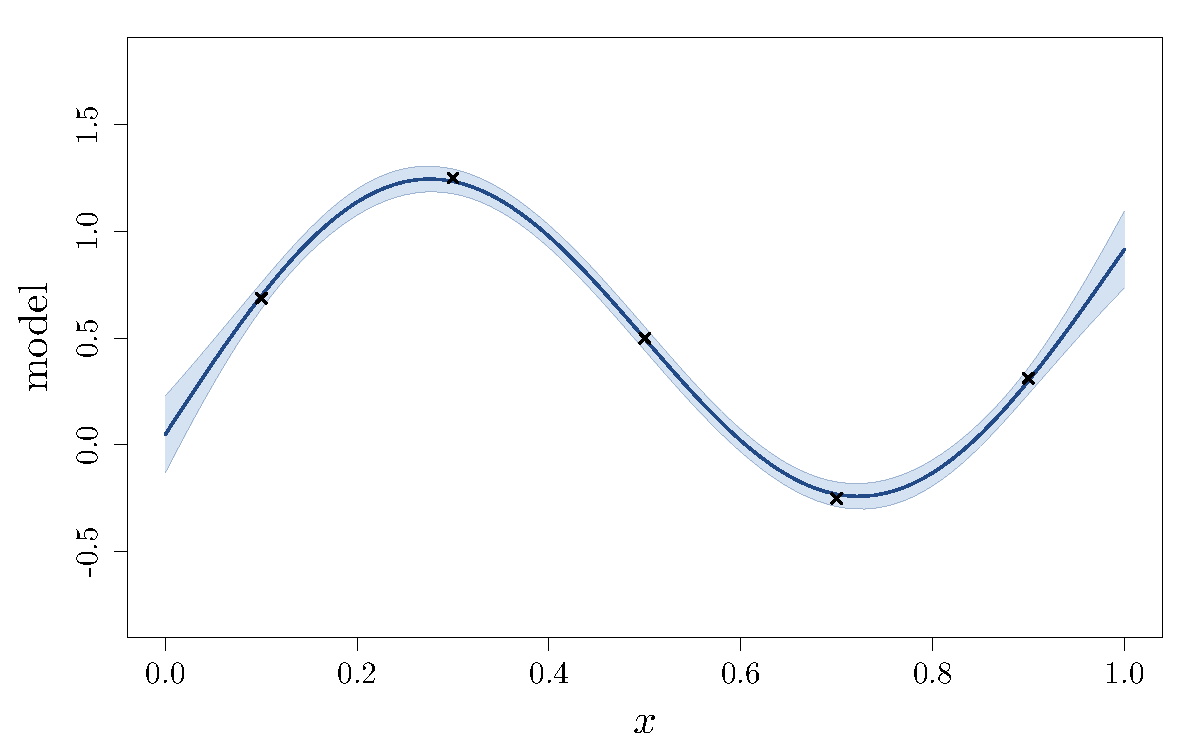
\includegraphics[height=5cm]{figures/R/model_0}
\end{center}
Today's question is: If the input points $X$ can be chosen, how can we obtain the best model?
\end{frame}

%%%%%%%%%%%%%%%%%%%%%%%%%%%%%%%%%%%%%%%%%%%%%%%%%%%%%%
\begin{frame}{}
\begin{exampleblock}{Motivating example}
Same number of points but different input locations \vspace{-2mm}
\begin{center}
  \begin{tabular}{cc}
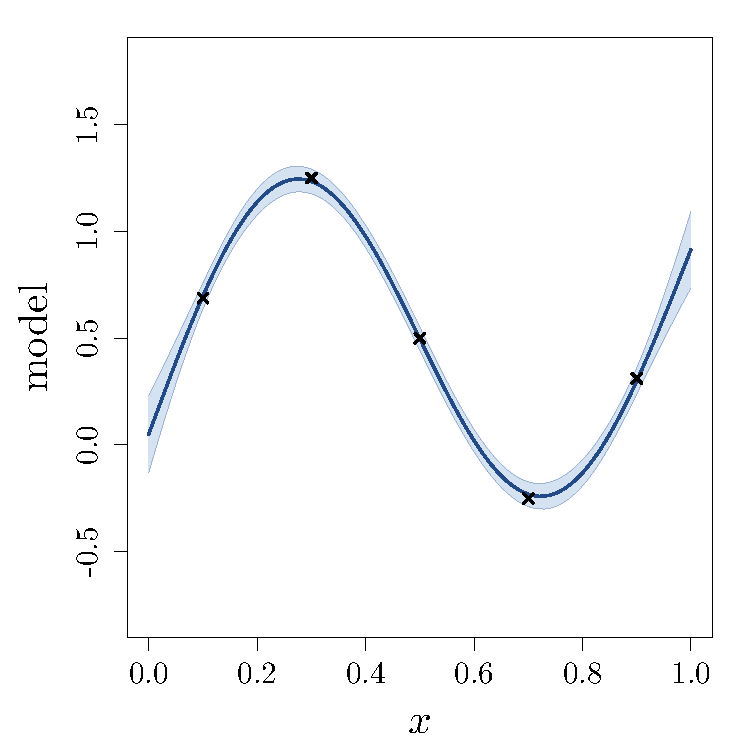
\includegraphics[height=5cm]{figures/R/model_1} & 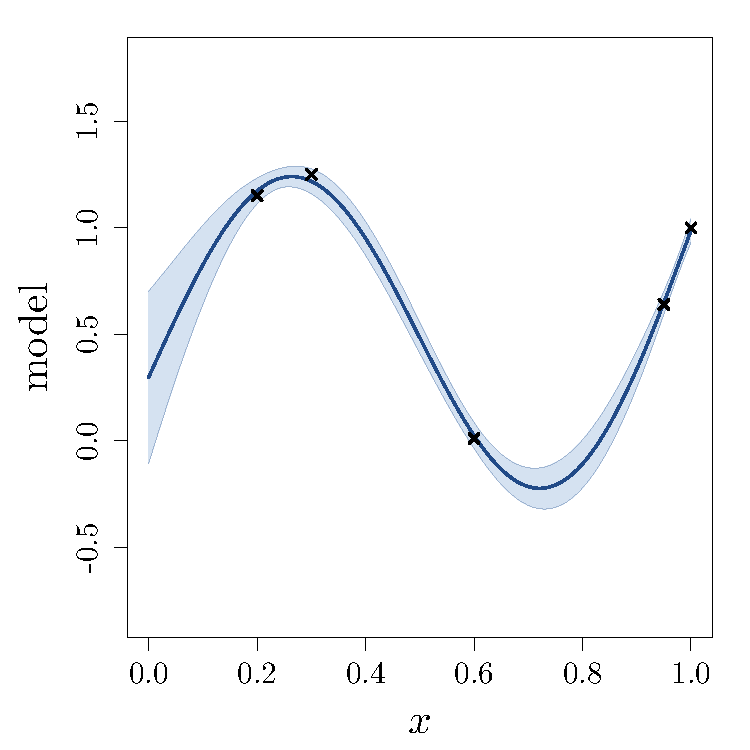
\includegraphics[height=5cm]{figures/R/model_2} \\
$RSS = 0.054$ & $RSS = 0.68$ \\
$IMSE = 0.001$ & $IMSE = 0.004$
  \end{tabular}
\end{center}
\end{exampleblock}
\end{frame}

%%%%%%%%%%%%%%%%%%%%%%%%%%%%%%%%%%%%%%%%%%%%%%%%%%%%%%
\begin{frame}{}
\structure{Outline of the lecture}
\vspace{0.2cm}
\begin{itemize}
	\item Classical designs
	\item Space filling designs
	\item Optimal design for a given model
\end{itemize}
\vspace{5mm}
This lecture is based on a course of Victor Picheny (INRA) at Mines St-\'Etienne.\\ 
\vspace{5mm}
We have focus in the past lecture on 1-dimensional examples, we have to bear in mind that the input space is often of high dimension ($d$ from 5 to 100).
\end{frame}

%%%%%%%%%%%%%%%%%%%%%%%%%%%%%%%%%%%%%%%%%%%%%%%%%%%%%%
\begin{frame}{}
Intuition is often misleading in high-dimension:
\begin{exampleblock}{Examples 1/2}
\begin{itemize}
	\item Points in the unit cube can be far away\\ \qquad $\rightarrow$ the diagonal of the unit cube is of length $\sqrt{d}$
	\item All the volume is near the domain boundaries \\ \qquad $\rightarrow$ let us consider a hypercube of size 0.9 included in the the unit cube:\vspace{5mm}
	\begin{center}
\includegraphics[height=4cm]{figures/latexdraw/volumedim} \quad
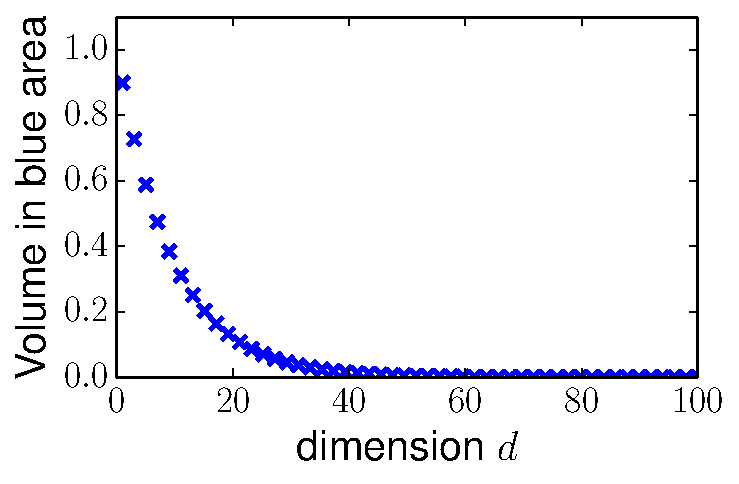
\includegraphics[height=3.5cm]{figures/python/spf_volume}
\end{center}
\end{itemize}	
\end{exampleblock}
\end{frame}

%%%%%%%%%%%%%%%%%%%%%%%%%%%%%%%%%%%%%%%%%%%%%%%%%%%%%%
\begin{frame}{}
Intuition is often misleading in high-dimension:
\begin{exampleblock}{Examples 2/2}
\begin{itemize}
	\item The number of vertices of an hypercube increases faster than we usually think
\end{itemize}	
\begin{columns}[c]
\column{5.5cm}
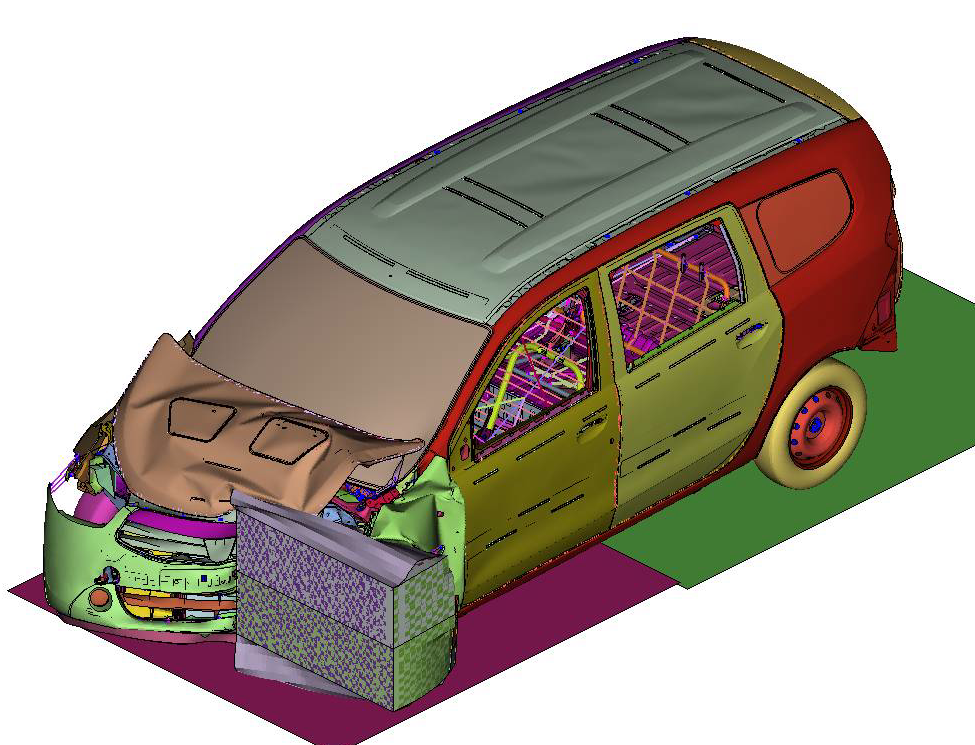
\includegraphics[height=4.5cm]{figures/crashtest} 
\column{5cm}
Testing all combinations of min and max input values for the 50 parameters would require... \pause
$$\mathbf{d=50 \ \Rightarrow \ 2^d \approx 1.e15 \ days}$$
\textbf{(3000 times the age of the universe)}\\
\end{columns}
\end{exampleblock}
\end{frame}

%%%%%%%%%%%%%%%%%%%%%%%%%%%%%%%%%%%%%%%%%%%%%%%%%%%%%%
%%%%%%%%%%%%%%%%%%%%%%%%%%%%%%%%%%%%%%%%%%%%%%%%%%%%%%
\section[Classical DoE]{Classical designs}
\subsection{}

%%%%%%%%%%%%%%%%%%%%%%%%%%%%%%%%%%%%%%%%%%%%%%%%%%%%%%
\begin{frame}{One at a time design}
An intuitive way to check the influence of various variables is to make them change one at the time.
\begin{itemize}
	\item All variables are fixed at a reference value (0 for example)
	\item One variable is changed at a time to see if there is an influence
\end{itemize}
\vspace{5mm}
\begin{example}
\begin{columns}[c]
\column{5cm}
\begin{center}
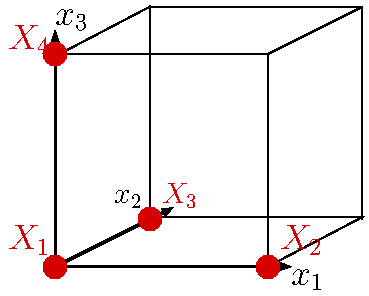
\includegraphics[width=4cm]{figures/latexdraw/1atatime}
\end{center}
\column{5cm}
\begin{center}
  \begin{tabular}{|c|ccc|}
  \hline
  point & $x_1$ & $x_2$ & $x_3$ \\ \hline
  $X_1$ & 0 & 0 & 0 \\
  $X_2$ & 1 & 0 & 0 \\
  $X_3$ & 0 & 1 & 0 \\
  $X_4$ & 0 & 0 & 1 \\ \hline
  \end{tabular}
\end{center}
\end{columns}
\end{example}
\end{frame}

%%%%%%%%%%%%%%%%%%%%%%%%%%%%%%%%%%%%%%%%%%%%%%%%%%%%%%
\begin{frame}{}
\textbf{pros and cons of this kind of design}:
\begin{itemize}
  \item[+] require only $d+1$ observations
  \item[+] are easy to interpret
  \item[] \vspace{-4mm}
  \item[$-$] they can only see linear effects: 
  \begin{center}
  $m(x)=\beta_0 + \beta_1 x_1 + \beta_2 x_2 + \beta_3 x_3$
  \end{center}
  \item[$-$] they do not cover the space
\end{itemize}
\vspace{5mm}
\begin{exampleblock}{Exercise}
How can this kind of design be adapted to estimate quadratic effect?
\end{exampleblock}
\end{frame}

%%%%%%%%%%%%%%%%%%%%%%%%%%%%%%%%%%%%%%%%%%%%%%%%%%%%%%
\begin{frame}{}
\begin{exampleblock}{Solution}
Quadratic effects can be estimated with either
\begin{center}
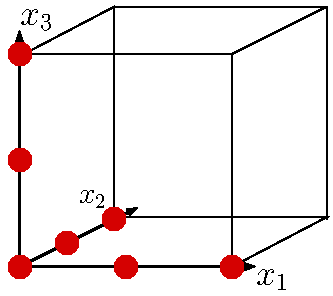
\includegraphics[width=4.5cm]{figures/latexdraw/1atatime1} \hspace{10mm}
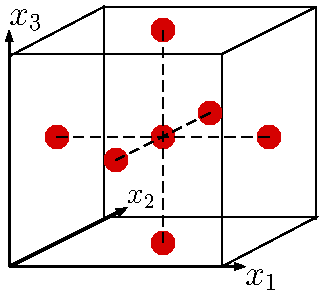
\includegraphics[width=4.5cm]{figures/latexdraw/1atatime2}
\end{center}
we sometime talk about ``star shaped'' design.
\end{exampleblock}
\end{frame}

%%%%%%%%%%%%%%%%%%%%%%%%%%%%%%%%%%%%%%%%%%%%%%%%%%%%%%
\begin{frame}{Factorial designs}
The principle of factorial design is to consider all combinations for $x_i \in \{0,1\}$:
\vspace{5mm}
\begin{columns}[c]
\column{4cm}
\begin{center}
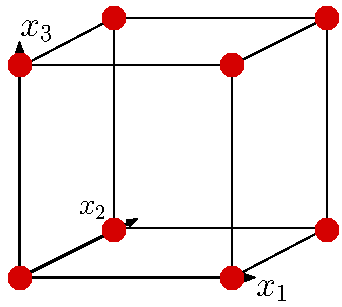
\includegraphics[width=4cm]{figures/latexdraw/factorial}
\end{center}
\column{6cm}
\begin{itemize}
	\item[\textbf{pros}] They allow to get all interaction terms:
\end{itemize}
	$$\beta_0 + \sum_k \beta_k x_k + \sum_{j,k} \beta_{j,k} x_j x_k  + \beta_{1,2,3} x_1 x_2 x_3$$		
\begin{itemize}
	\item[\textbf{cons}] The number of evaluation is unrealistic when $d$ is large  
\end{itemize}
\end{columns}
\end{frame}

%%%%%%%%%%%%%%%%%%%%%%%%%%%%%%%%%%%%%%%%%%%%%%%%%%%%%%
\begin{frame}{Factorial designs}
It is also possible to build factorial designs with $k$ levels:
\begin{center}
\includegraphics[width=5cm]{figures/latexdraw/factorial3levels}
\end{center}
This allows to compute quadratic effects but the number of evaluations $k^d$ is even less realistic...
\end{frame}

%%%%%%%%%%%%%%%%%%%%%%%%%%%%%%%%%%%%%%%%%%%%%%%%%%%%%%
\begin{frame}{}
\textbf{Conclusion on classical designs:}\\
\structure{\textbf{pros:}}\\
\quad Easy to use\\
\quad adapted to continuous or discrete variables\\
\quad Can be combined (star + factorial for example)\\
\quad Well suited (often optimal) for linear regression\\
\vspace{5mm}
\structure{\textbf{cons:}}\\
\quad Number of evaluation is not flexible\\
\quad Number of evaluation too large in high dimension\\
\quad Points are on top of each other when projected
\end{frame}

%%%%%%%%%%%%%%%%%%%%%%%%%%%%%%%%%%%%%%%%%%%%%%%%%%%%%%
\begin{frame}{projection issues}
Why don't we want points to be superimposed when projected?\\
If one of the variables has no influence, most observations become redundant...
\begin{center}
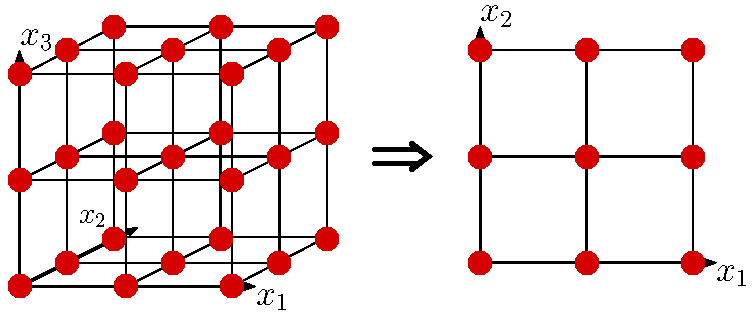
\includegraphics[height=4.5cm]{figures/latexdraw/factorialprojection}
\end{center}
From 27 observations, we end up with only 9...
\end{frame}

%%%%%%%%%%%%%%%%%%%%%%%%%%%%%%%%%%%%%%%%%%%%%%%%%%%%%%
%%%%%%%%%%%%%%%%%%%%%%%%%%%%%%%%%%%%%%%%%%%%%%%%%%%%%%
\section{Space filling DoE}
\subsection{}


%%%%%%%%%%%%%%%%%%%%%%%%%%%%%%%%%%%%%%%%%%%%%%%%%%%%%%
\begin{frame}{}
We are now looking for designs of experiments that:
\begin{itemize}
	\item are not model oriented
	\item give information about every domain of the input space
	\item have good projection on subspaces
	\item have a flexible number of points
\end{itemize}
\end{frame}

%%%%%%%%%%%%%%%%%%%%%%%%%%%%%%%%%%%%%%%%%%%%%%%%%%%%%%
\begin{frame}{}
How can we evaluate if a set of points fills the space?\\ \vspace{5mm}
\textbf{1. Compute the distance between points}\\
\begin{itemize}
	\item[maximin] the minimum distance between two points of the design should be large:
	$$\text{Optimisation problem is: \quad} \max_{X_1,\dots,X_n} [ \min_{i \neq j} dist(X_i,X_j) ]$$
	\item[minimax] the maximum distance between any point of the space and closest design point should be small:
	$$\text{Optimisation problem is: \quad} \min_{X_1,\dots,X_n} (\max_{x \in D} [ \min_i dist(x,X_i) ])$$
\end{itemize}
The second criterion is much more difficult to optimise
\end{frame}

%%%%%%%%%%%%%%%%%%%%%%%%%%%%%%%%%%%%%%%%%%%%%%%%%%%%%%
\begin{frame}{}
These criteria can be illustrated on a simple 2-dimensional example
\begin{center}
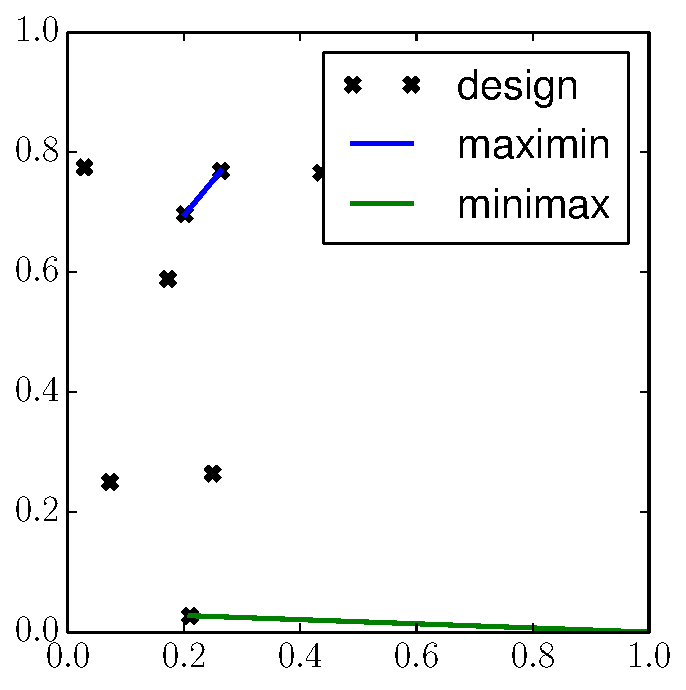
\includegraphics[height=6.5cm]{figures/python/spf_minimaxmaximin}
\end{center}
\end{frame}

%%%%%%%%%%%%%%%%%%%%%%%%%%%%%%%%%%%%%%%%%%%%%%%%%%%%%%
\begin{frame}{}
\textbf{2. Compare the distribution with an uniform distribution}\\
\structure{Discrepency} is a measure of non uniformity. It compares the number of points in a hyper-rectangle with the expected number of samples from a uniform distribution
\vspace{-2mm}
\begin{columns}[c]
\column{4cm}
\begin{center}
\includegraphics[height=4cm]{figures/latexdraw/discrepency}
\end{center}
\column{6cm}
The probability for a uniform variable to be in $R$ is 0.22 and we observe an empirical probability of $2/11$. The discrepancy (w.r.t. $R$) is then:
$$D_R = |0.22-2/11| = 0.038$$
\end{columns}
\vspace{2mm}
Discrepency is defined as the sup of the distance between the empirical and analytical cdf.
\end{frame}

%%%%%%%%%%%%%%%%%%%%%%%%%%%%%%%%%%%%%%%%%%%%%%%%%%%%%%
\begin{frame}{}
Discrepency is often computed by fixing:
\begin{itemize}
 	\item one of the hyper-rectangle summit at the origin
 	\item the hyper-rectangle centre at the domain centre
 \end{itemize} 
\begin{center}
\includegraphics[height=4.5cm]{figures/latexdraw/discrepency3}
\end{center}
The maximum is located where the rectangle is tangent to points\\
$\rightarrow$ The optimisation is over a finite space
\end{frame}

%%%%%%%%%%%%%%%%%%%%%%%%%%%%%%%%%%%%%%%%%%%%%%%%%%%%%%
\begin{frame}{}
We will discuss three types of space filling designs:
\begin{itemize}
	\item Latin hypercubes
	\item low discrepancy sequences
	\item centroidal Voronoi tesselations
\end{itemize}
\end{frame}

%%%%%%%%%%%%%%%%%%%%%%%%%%%%%%%%%%%%%%%%%%%%%%%%%%%%%%
\begin{frame}{Latin hypercubes}
\textbf{Latin hypercubes} are designs where the domain is sliced in $n^d$ blocks and where there is only one point per `column':
\begin{center}
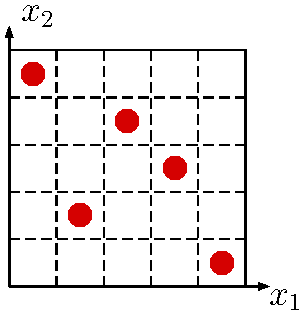
\includegraphics[height=5cm]{figures/latexdraw/lhs1}
\end{center}
These designs have good projection properties
\end{frame}


%%%%%%%%%%%%%%%%%%%%%%%%%%%%%%%%%%%%%%%%%%%%%%%%%%%%%%
\begin{frame}{}
A well known example of LHS in 2D is... \pause Sudoku
\vspace{5mm}
\begin{center}
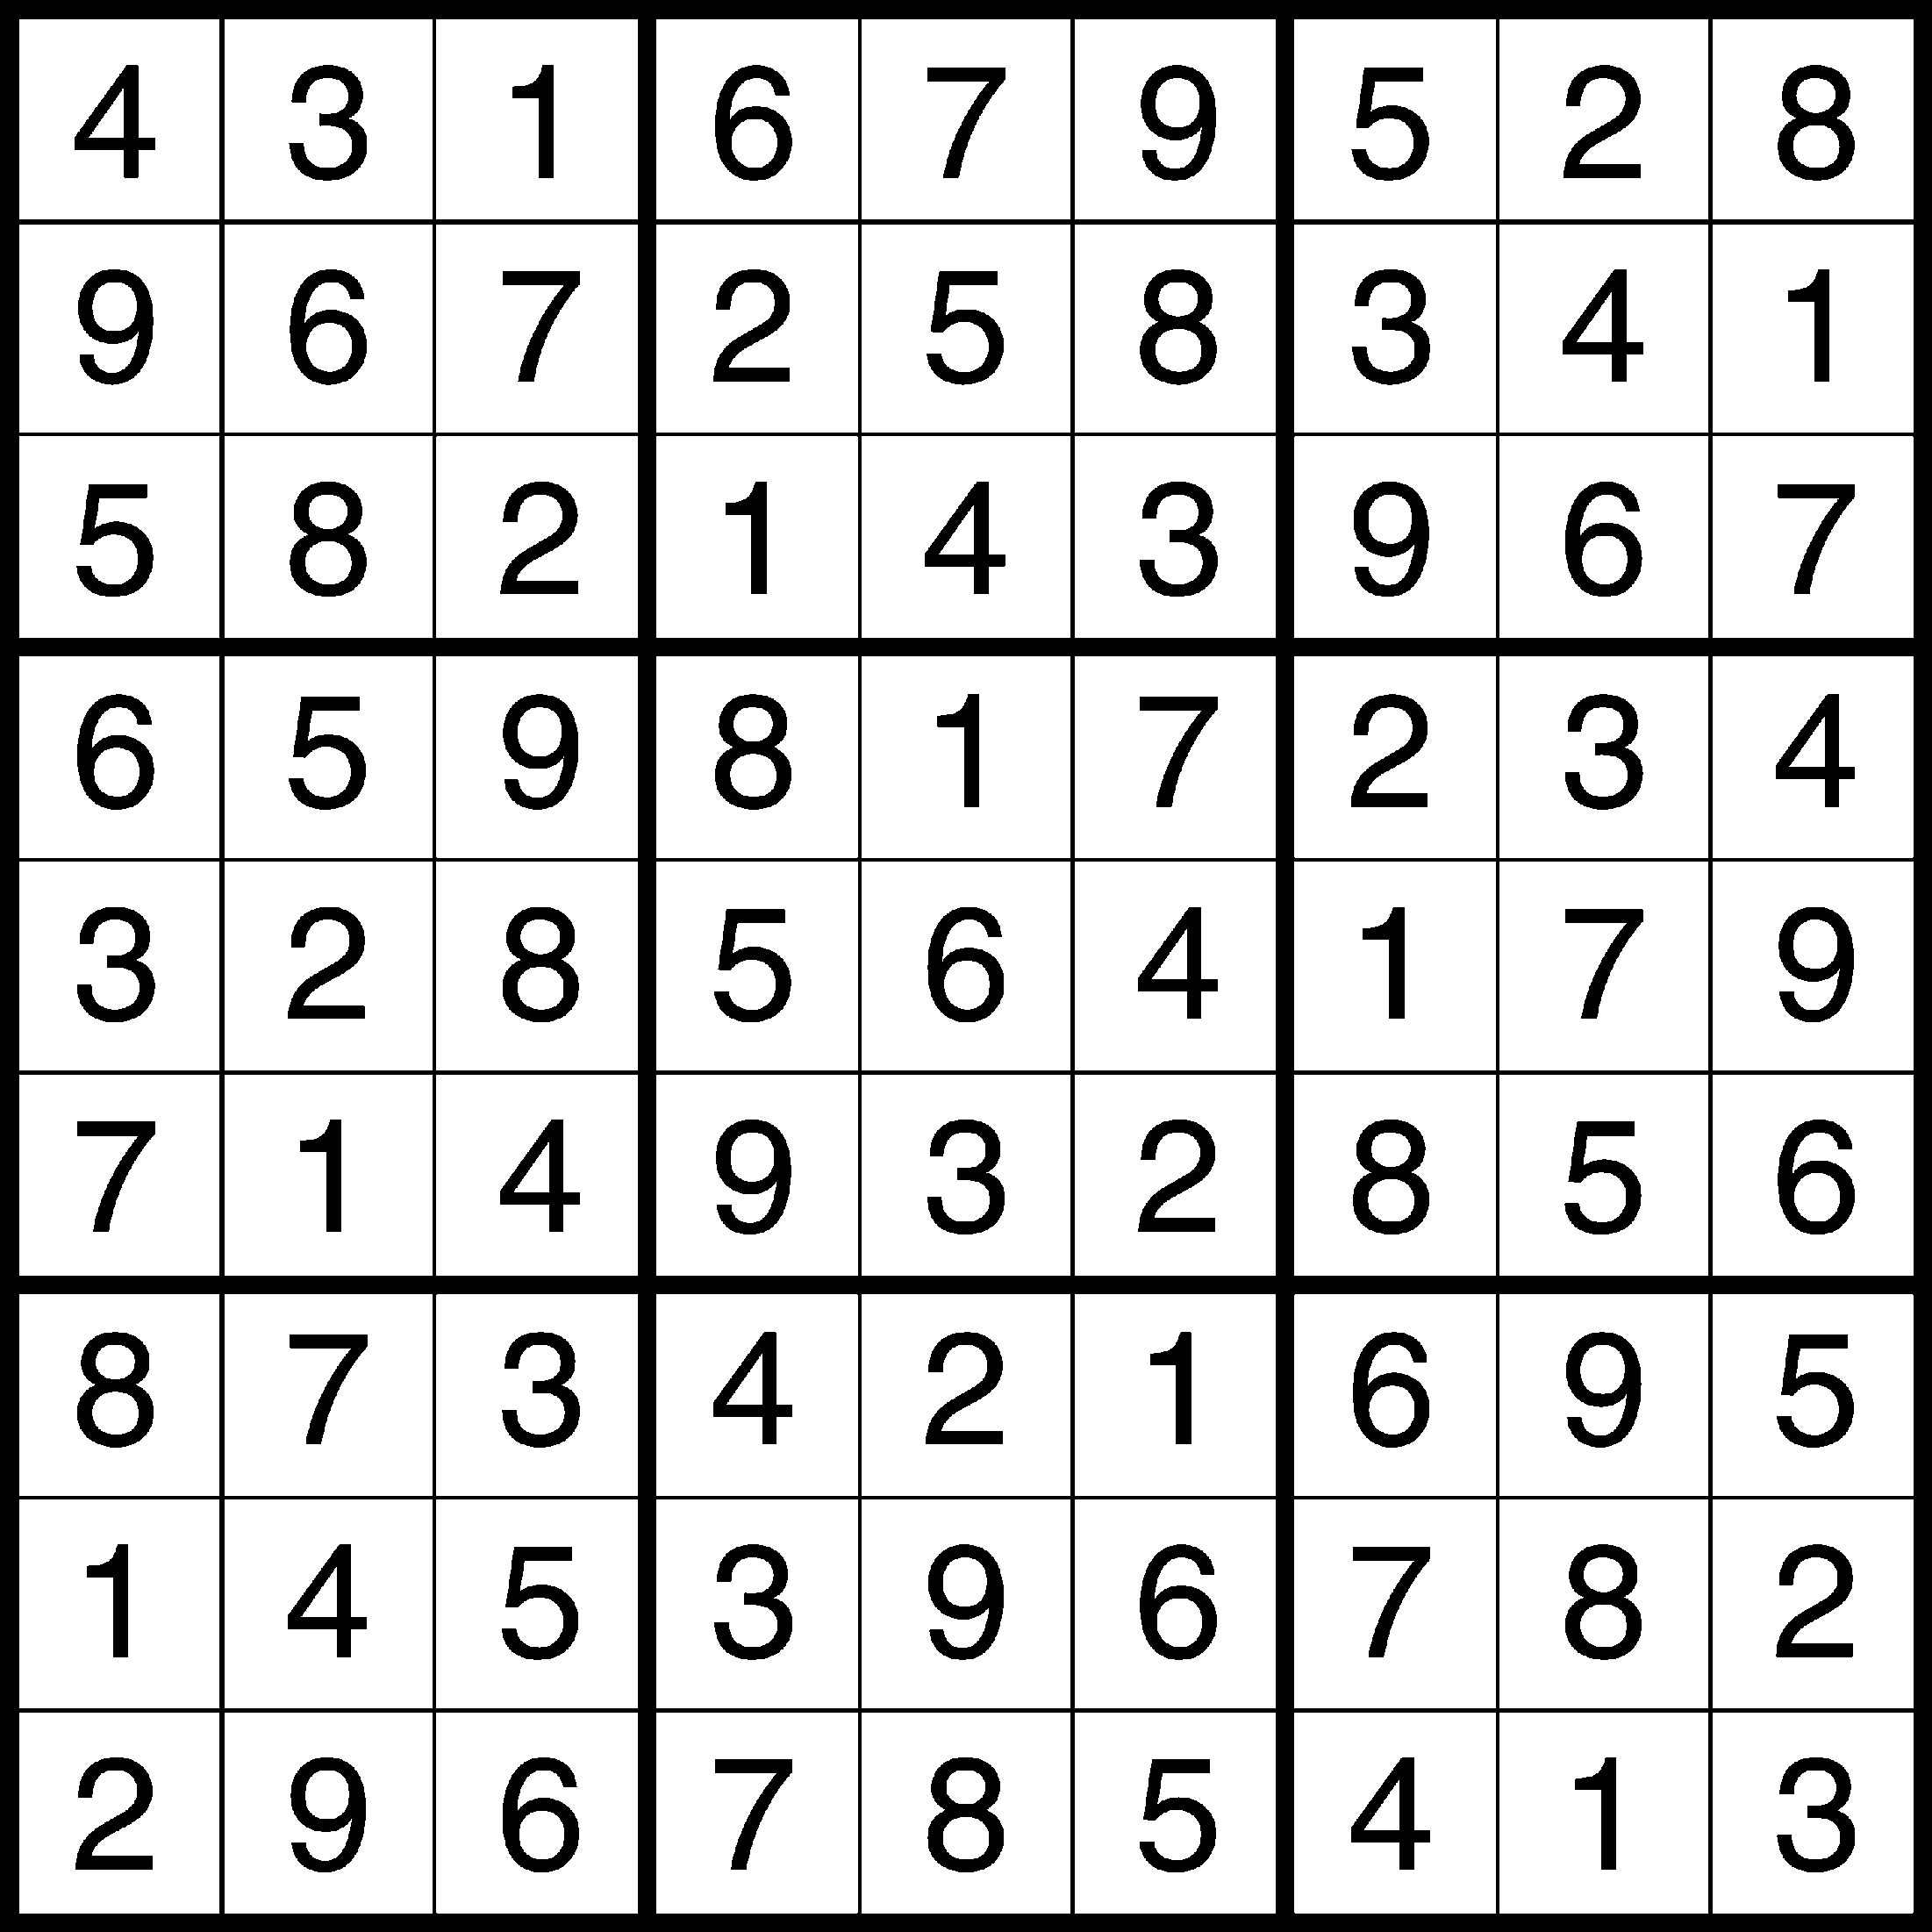
\includegraphics[height=5cm]{figures/sudoku}
\end{center}
\end{frame}

%%%%%%%%%%%%%%%%%%%%%%%%%%%%%%%%%%%%%%%%%%%%%%%%%%%%%%
\begin{frame}{}
If we focus on one digit (say $4$), we obtain a LHD:
\vspace{2mm}
\begin{center}
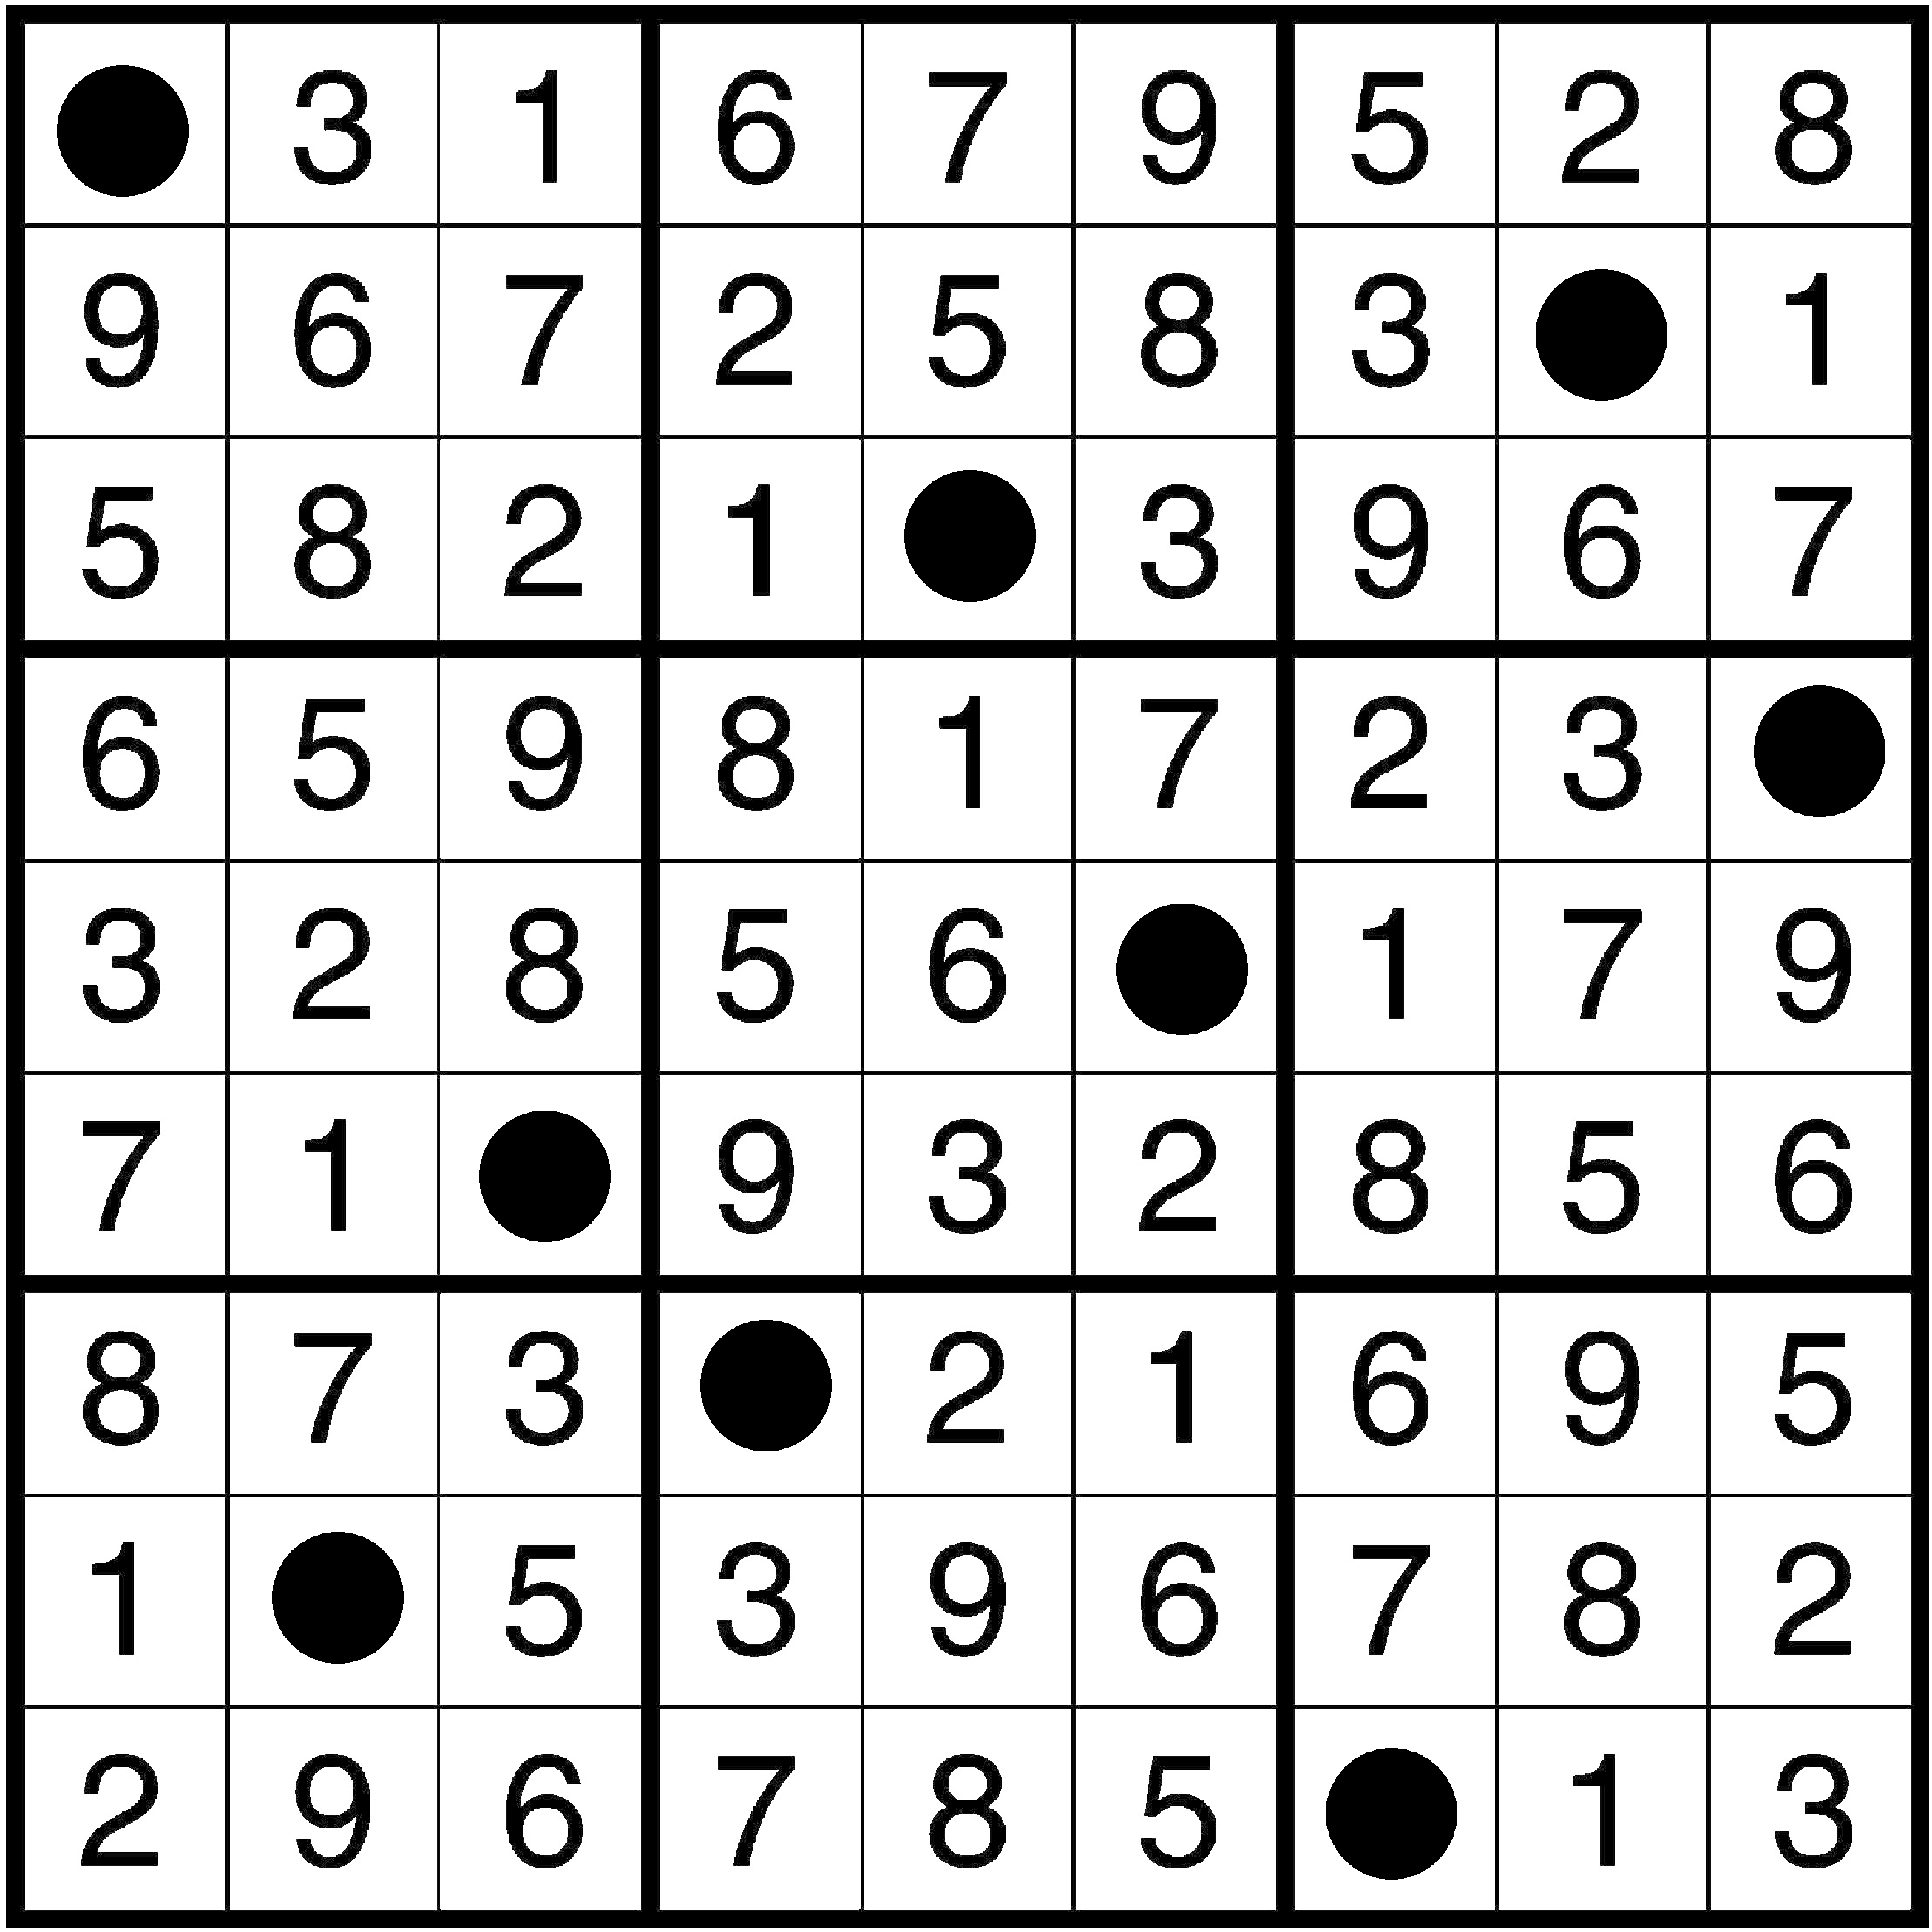
\includegraphics[height=5cm]{figures/latexdraw/sudoku}
\end{center}
Sudoku have more properties that LHD: the generalisation is called \textbf{orthogonal array}.
\end{frame}

%%%%%%%%%%%%%%%%%%%%%%%%%%%%%%%%%%%%%%%%%%%%%%%%%%%%%%
\begin{frame}{}
Latin hypercubes do not necessarily cover the space very well...
\begin{center}
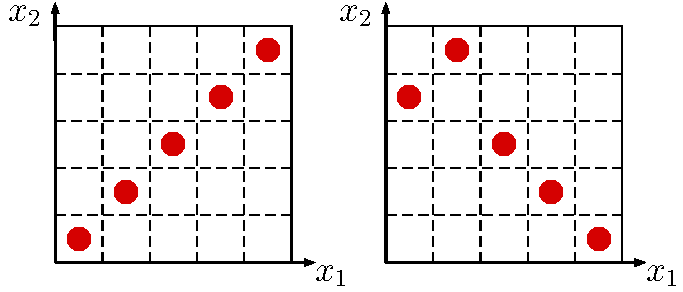
\includegraphics[height=4.5cm]{figures/latexdraw/lhs2}
\end{center}
They have to be combined with a criterion such as maximin.
\end{frame}

%%%%%%%%%%%%%%%%%%%%%%%%%%%%%%%%%%%%%%%%%%%%%%%%%%%%%%
\begin{frame}{}
\begin{exampleblock}{Exercise}
\begin{itemize}
	\item Generate a 5 points LH in dimension 3.
	\item How would you program a function $LHD(n,d)$? 
\end{itemize}
\end{exampleblock}
\end{frame}

%%%%%%%%%%%%%%%%%%%%%%%%%%%%%%%%%%%%%%%%%%%%%%%%%%%%%%
\begin{frame}{}
\begin{exampleblock}{Exercise}
How would you optimize LHD?
\end{exampleblock}
\pause
the coordinates of two points can be exchanged:\\
\vspace{4mm}
\begin{center}
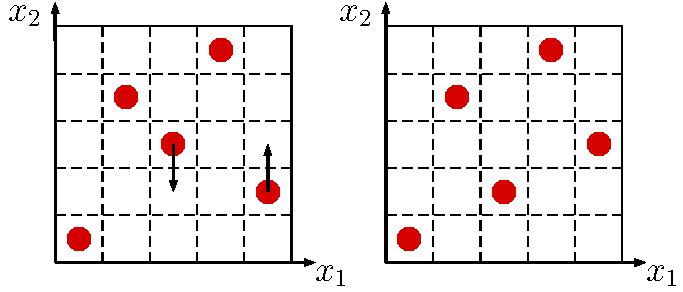
\includegraphics[height=4.5cm]{figures/latexdraw/lhs3}
\end{center}
\end{frame}

%%%%%%%%%%%%%%%%%%%%%%%%%%%%%%%%%%%%%%%%%%%%%%%%%%%%%%
\begin{frame}{}
LHD optimization with simulated annealing:\\
\vspace{4mm}
\textbf{Morris and Mitchell Algorithm}\\
\vspace{2mm}
\begin{itemize}
	\item[1] Generate LHD
	\item[2] find ``bad'' points according to maximin
	\item[3] choose randomly a column of this critical point and exchange it with an randomly selected other point
	\item[4] \qquad if the criteria is improved, the modification is accepted
	\item[5] \qquad otherwise, it is accepted with a probability of $$\exp \left(\frac{maximin_{new}-maximin_{old}}{T}\right)$$
	\end{itemize}
\end{frame}



%%%%%%%%%%%%%%%%%%%%%%%%%%%%%%%%%%%%%%%%%%%%%%%%%%%%%%
\begin{frame}{Low discrepancy sequences}
\textbf{Low discrepancy sequences} are deterministic sequences that converge toward the uniform distribution. 
\begin{itemize}
	\item They cover the space quickly and evenly
	\item They are easy to build
	\item It is easy to add new points
\end{itemize}
\vspace{5mm}
Many low discrepancy sequences can be found in the literature: Halton, Hammerley, Sobol', Faure, van der Corput, ...
\end{frame}

%%%%%%%%%%%%%%%%%%%%%%%%%%%%%%%%%%%%%%%%%%%%%%%%%%%%%%
\begin{frame}{}
\begin{example}[Halton sequence]
	Let $a$ and $b$ be two integers with no common dividers (say 2 and 3). The $x_1$ and $x_2$ coordinates of the Halton sequence are:
	\begin{equation*}
		\begin{split}
			x_1 &= 1/2,\ 1/4,\ 3/4,\ 1/8,\ 5/8,\ 3/8,\ 7/8,\ 1/16,\ 9/16, \dots\\
			x_2 &= 1/3,\ 2/3,\ 1/9,\ 4/9,\ 7/9,\ 2/9,\ 5/9,\ 8/9,\ 1/27, \dots
		\end{split}
	\end{equation*}
\begin{center}
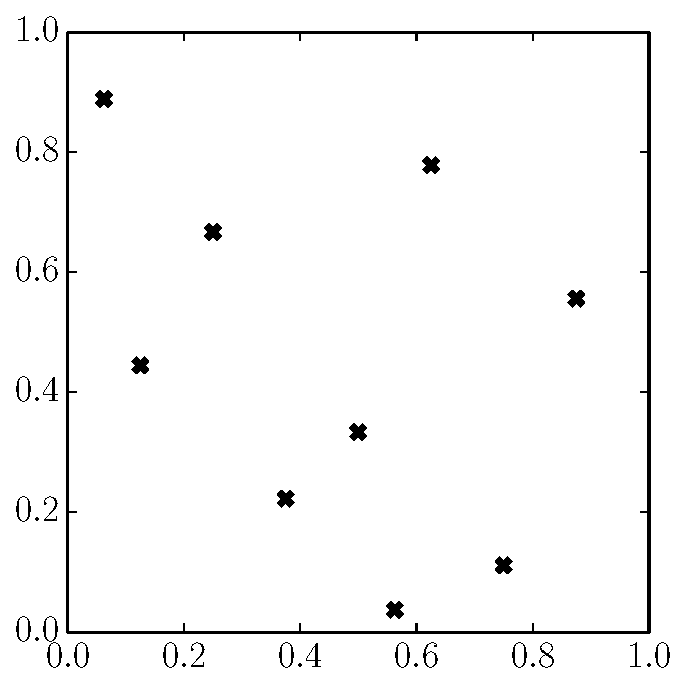
\includegraphics[height=4.5cm]{figures/python/spf_halton}
\end{center}

\end{example}
\end{frame}

%%%%%%%%%%%%%%%%%%%%%%%%%%%%%%%%%%%%%%%%%%%%%%%%%%%%%%
\begin{frame}{}
\begin{example}[Halton sequence]
\begin{center}
  \begin{tabular}{cc}
Halton Sequence & uniform pseudo random \\
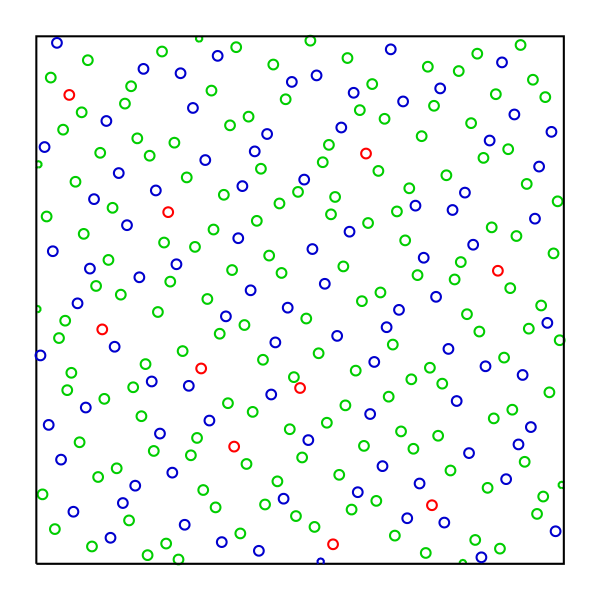
\includegraphics[height=5cm]{figures/Halton} & 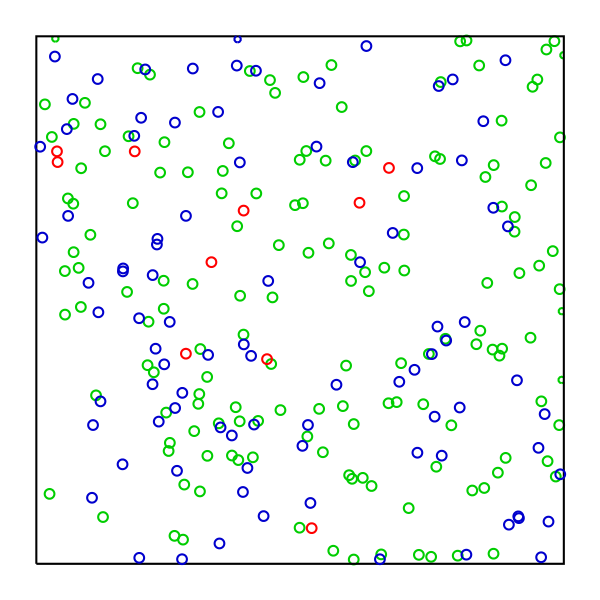
\includegraphics[height=5cm]{figures/random}
  \end{tabular}
 source: wikipedia 
\end{center}
\end{example}
\end{frame}

%%%%%%%%%%%%%%%%%%%%%%%%%%%%%%%%%%%%%%%%%%%%%%%%%%%%%%
\begin{frame}{}
Issues with low discrepancy sequences:
\begin{itemize}
	\item[$-$] there can be alignments when projected 
	\item[$-$] there can be holes in subspaces
	\item[$-$] points may be aligned (Example: 16 first points in basis (17,18))
\end{itemize}
\end{frame}

%%%%%%%%%%%%%%%%%%%%%%%%%%%%%%%%%%%%%%%%%%%%%%%%%%%%%%
\begin{frame}{Centroidal Voronoi Tesselations}
Given a set of generative points $X$, the \textbf{Voronoi Tesselations} (or Voronoi cells) associated to the point $X_i$ is the region of the space such that $X_i$ is the closest point from the set:
\begin{center}
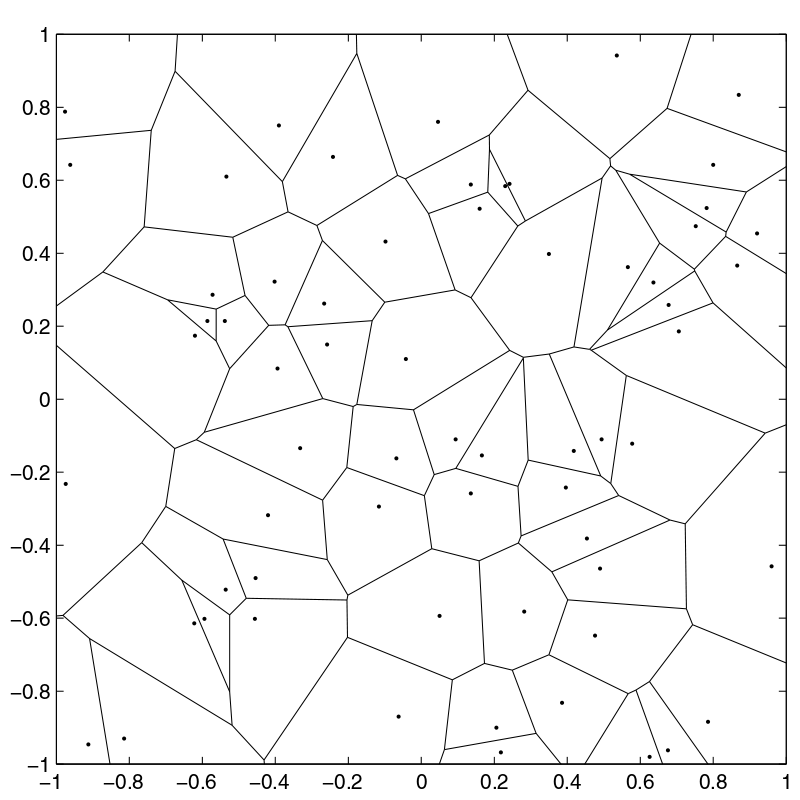
\includegraphics[height=5cm]{figures/VT}
\end{center}
Source: Q. Du et Al., \emph{Centroidal Voronoi Tessellations: Applications and Algorithms}, SIAM Review, 41-4, 1999.
\end{frame}

%%%%%%%%%%%%%%%%%%%%%%%%%%%%%%%%%%%%%%%%%%%%%%%%%%%%%%
\begin{frame}{}
\textbf{Centroidal Voronoi Tesselations (CVT)} is a special case of Voronoi Tesselations where the generative points correspond to the centre of mass of the cells
\begin{center}
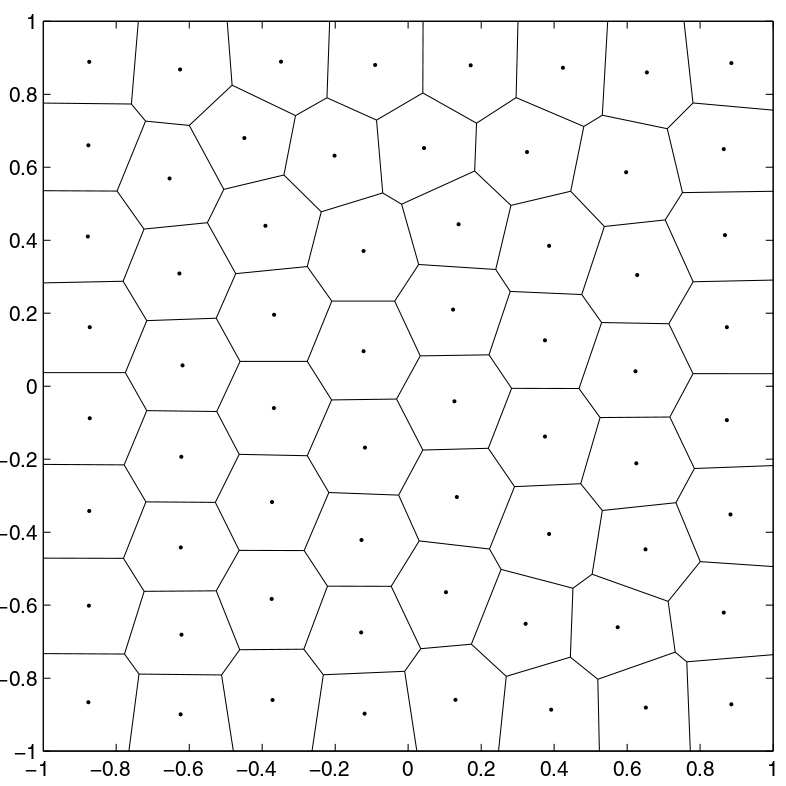
\includegraphics[height=5cm]{figures/CVT}
\end{center}
Source: Q. Du et Al., \emph{Centroidal Voronoi Tessellations: Applications and Algorithms}, SIAM Review, 41-4, 1999.
\end{frame}

%%%%%%%%%%%%%%%%%%%%%%%%%%%%%%%%%%%%%%%%%%%%%%%%%%%%%%
\begin{frame}{}

Properties of CVT:
\begin{itemize}
	\item Each point of the space is close to one generative points
	\item The generative points cover the space
\end{itemize}
$\Rightarrow$ The generative points of CVT can be used as design of experiment.
\end{frame}

%%%%%%%%%%%%%%%%%%%%%%%%%%%%%%%%%%%%%%%%%%%%%%%%%%%%%%
\begin{frame}{Generating CVT }
\textbf{1. Lloyd's Algorithm}
\begin{itemize}
	\item[1] Initialize $X$ as a set of $n$ points
	\item[2] While $i<nb\_iter$ 
	\item[3] \qquad Compute the Voronoi diagram of $X$
	\item[4] \qquad X = centre of mass of each cell
\end{itemize}
\begin{center}
  \begin{tabular}{cccc}
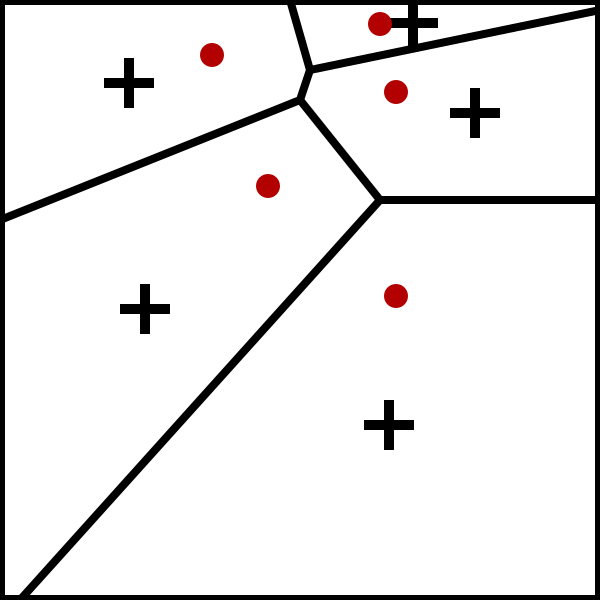
\includegraphics[height=2.4cm]{figures/Lloyds1}&
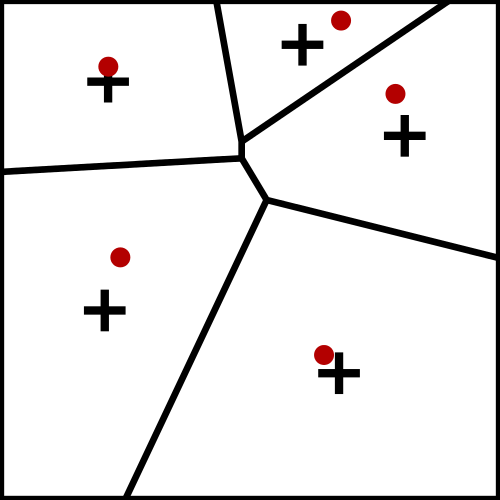
\includegraphics[height=2.4cm]{figures/Lloyds2}&
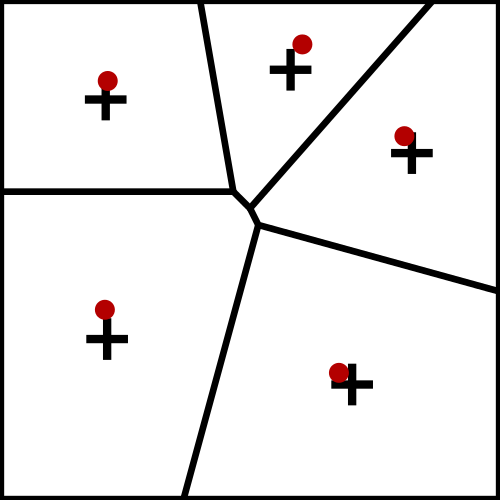
\includegraphics[height=2.4cm]{figures/Lloyds3}&
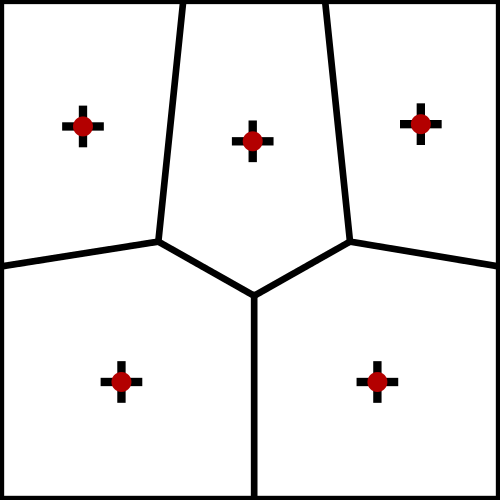
\includegraphics[height=2.4cm]{figures/Lloyds15}\\
iteration 1 & iteration 2 &iteration 3 &iteration 15
  \end{tabular}
\end{center}
source: ``Lloyd's algorithm'' wikipedia page
\end{frame}

%%%%%%%%%%%%%%%%%%%%%%%%%%%%%%%%%%%%%%%%%%%%%%%%%%%%%%
\begin{frame}{Generating CVT }
\textbf{2. k-means}\\
This algorithm is very similar to Lloyd but it uses a large set of points covering the input space instead of the full continuous domain:
\begin{center}
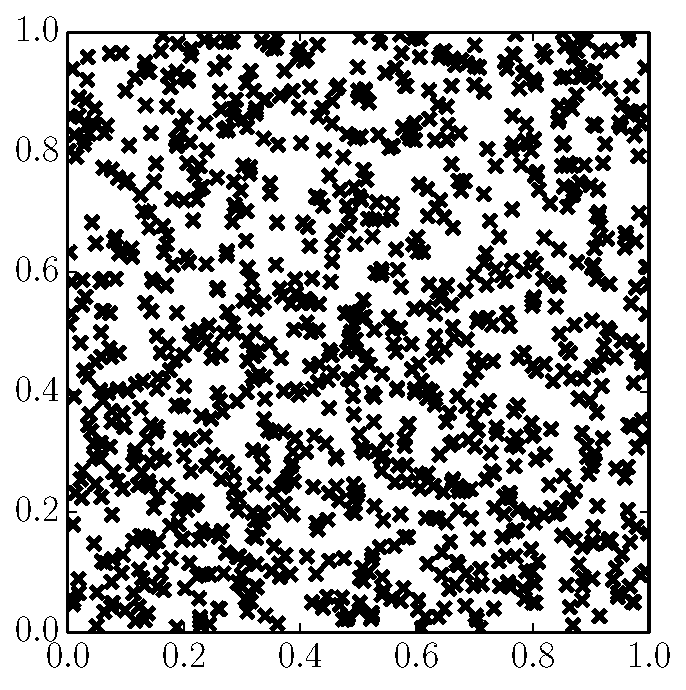
\includegraphics[height=4.5cm]{figures/python/spf_kmeans1}

\includegraphics[height=4.5cm]{figures/Rightarrow}
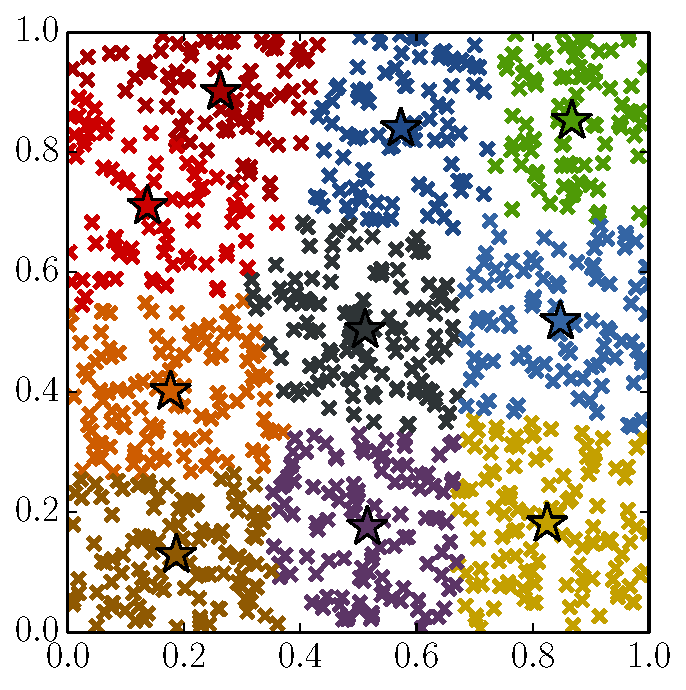
\includegraphics[height=4.5cm]{figures/python/spf_kmeans2}
\end{center}
\end{frame}

%%%%%%%%%%%%%%%%%%%%%%%%%%%%%%%%%%%%%%%%%%%%%%%%%%%%%%
\begin{frame}{Generating CVT }
\textbf{3. McQueen algorithm}\\
\vspace{5mm}
This algorithm is much faster than the previous ones and gives a good approximation
\begin{itemize}
	\item[1] Initialize $X$ as a set of $n$ points
	\item[2] Initialize $k$ as a vector of 1 with length $n$
	\item[3] While $i<nb\_iter$ 
	\item[4] \qquad generate one random point $z$ in the input space
	\item[5] \qquad find the $X_i$ closest to $z$
	\item[6] \qquad update $X_i = \frac{k_i x + z}{k_i+1}$
	\item[7] \qquad $k_i =k_i+1$
\end{itemize}
\end{frame}

%%%%%%%%%%%%%%%%%%%%%%%%%%%%%%%%%%%%%%%%%%%%%%%%%%%%%%
\begin{frame}{Generating CVT }
\textbf{3. McQueen algorithm}\\
We obtain the following design:
\begin{center}
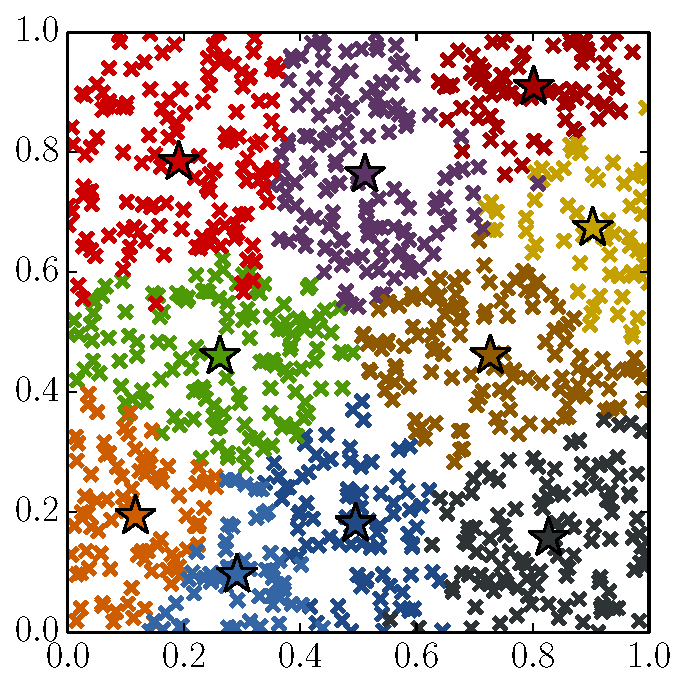
\includegraphics[height=5cm]{figures/python/spf_McQueen}
\end{center}
\end{frame}

%%%%%%%%%%%%%%%%%%%%%%%%%%%%%%%%%%%%%%%%%%%%%%%%%%%%%%
\begin{frame}{}
CVT are not unique:
\begin{center}
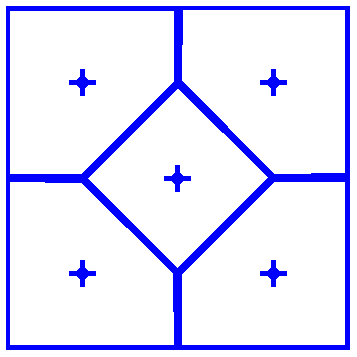
\includegraphics[height=3cm]{figures/CVT1} \qquad
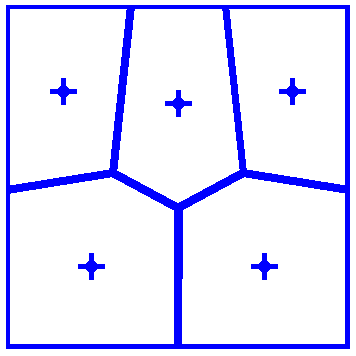
\includegraphics[height=3cm]{figures/CVT2} \qquad
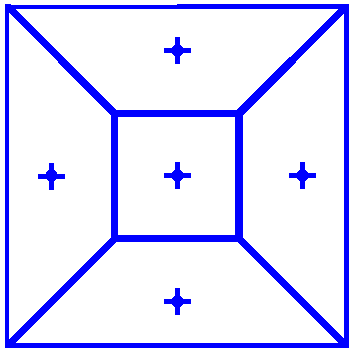
\includegraphics[height=3cm]{figures/CVT3}
\end{center}
 source: wikipedia page ``Centroidal Voronoi Tesselations''
\end{frame}

%%%%%%%%%%%%%%%%%%%%%%%%%%%%%%%%%%%%%%%%%%%%%%%%%%%%%%
%%%%%%%%%%%%%%%%%%%%%%%%%%%%%%%%%%%%%%%%%%%%%%%%%%%%%%
\section[Optimal DoE for LR]{Optimal design for regression}
\subsection{}

%%%%%%%%%%%%%%%%%%%%%%%%%%%%%%%%%%%%%%%%%%%%%%%%%%%%%%
\begin{frame}{Design for regression models}
As detailed in lecture 1, the expression of the mean and variance of a linear regression model are:
\begin{equation*}
	\begin{split}
		m(x) & = B(x) (B(X)^t B(X))^{-1} B(X)^t F\\
		v(x) & = \sigma^2 B(x) (B(X)^t B(X))^{-1} B(x)^t
	\end{split}
\end{equation*}
where $B$ is a set of basis functions, $X$ is the DoE, $F$ is the vector of observations and $\sigma^2$ is the variance of the observation noise.\\
\vspace{5mm}
What would be the designs such that:
\begin{itemize}
	\item $\hat{\beta}$ is a good estimate of $\beta$?
	\item the prediction variance is minimal?
\end{itemize}
\end{frame}

%%%%%%%%%%%%%%%%%%%%%%%%%%%%%%%%%%%%%%%%%%%%%%%%%%%%%%
\begin{frame}{}
\begin{exampleblock}{Exercise}
	We consider a linear regression model over $(0,1)$ with one basis function $b(x)=x$ and one observation $X_1$.
	\begin{enumerate}
	 	\item Give the expression of $m$ and $v$.
	 	\item What is the value of $x$ that minimises the maximum of $v$?
	 	\item Give the expression of the variance of $\hat{\beta}$.
	 	\item What is the value of $x$ that minimises it?
	 \end{enumerate} 
	What happen if we have two basis functions $b_0(x)=1$, $b_1(x)=x$ and two observations?
\end{exampleblock}
\end{frame}

%%%%%%%%%%%%%%%%%%%%%%%%%%%%%%%%%%%%%%%%%%%%%%%%%%%%%%
\begin{frame}{}
From the previous example, we can see that 
\begin{itemize}
	\item Minimising beta variance $\Leftrightarrow$ Minimising prediction variance
	\item $X$ only has an influence on the term $(B(X)^t B(X))^{-1}$, which is the covariance matrix of $\hat{\beta}$ (up to a $\sigma^2$ factor)
\end{itemize}
\vspace{5mm}
\begin{columns}[c]
\column{3cm}
We thus want to minimise this uncertainty.
\column{5cm}
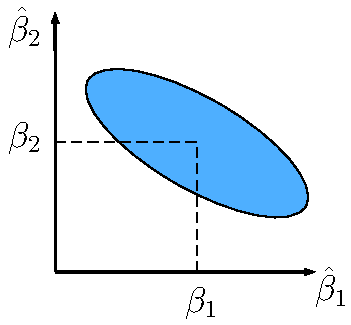
\includegraphics[height=4.5cm]{figures/latexdraw/optimalDoEreg}
\end{columns}
\end{frame}

%%%%%%%%%%%%%%%%%%%%%%%%%%%%%%%%%%%%%%%%%%%%%%%%%%%%%%
\begin{frame}{}
\textbf{Various criteria for the variability of the estimate:}
\begin{block}{D-optimality}
	The volume of the confidence ellipsoid is minimized
	$$ \min_X \mathrm{det} (B(X)^t B(X))^{-1} = \max \mathrm{det} B(X)^t B(X)$$
\end{block}
\begin{block}{A-optimality}
	The sum of the coefficients variance is minimized
	$$ \min_X \mathrm{tr} (B(X)^t B(X))^{-1} $$
\end{block}
\begin{block}{E-optimality}
	The maximum eigenvalue of $(B(X)^t B(X))^{-1}$ is minimized
	$$ \min_X \min_i \lambda_i \text{\qquad (where $\lambda_i$ is eigenvalue of $B(X)^t B(X))$}$$
\end{block}
\end{frame}

%%%%%%%%%%%%%%%%%%%%%%%%%%%%%%%%%%%%%%%%%%%%%%%%%%%%%%
\begin{frame}{}
\textbf{Various criteria for the prediction variance:}
\begin{block}{G-optimality}
	maximum of the prediction variance is minimized
	$$ \min_X \max_x \sigma^2 B(x) (B(X)^t B(X))^{-1} B(x)^t$$
\end{block}
\begin{block}{IMSE-optimality (or I-optimality)}
	the integrated variance is minimized
	$$ \min_X \int \sigma^2 B(x) (B(X)^t B(X))^{-1} B(x)^t \dx x$$
\end{block}
\end{frame}

%%%%%%%%%%%%%%%%%%%%%%%%%%%%%%%%%%%%%%%%%%%%%%%%%%%%%%
\begin{frame}{}
In practice, the optimization of these criterion is difficult:
\begin{itemize}
	\item Large number of variables ($n \times d$)
	\item multimodal function (lots of symmetries)
\end{itemize}
\vspace{10mm}
Some algorithms (such as Fedorov) are based on one at a time points replacement:
\begin{itemize}
 	\item[1.] Find the worst point in the Design
 	\item[2.] Find a critic region (large variance)
 	\item[3.] Replace the ``bad'' point by a point in the critic region 
 \end{itemize} 
\end{frame}

%%%%%%%%%%%%%%%%%%%%%%%%%%%%%%%%%%%%%%%%%%%%%%%%%%%%%%
\begin{frame}{}
\begin{block}{Equivalence theorem (Kiefer and Wolfowitz)}
The three conditions are equivalent
\begin{itemize}
 	\item A design is D-optimal
 	\item A design is G-optimal
 	\item The maximum prediction variance is $p$ 
 \end{itemize} 
\end{block}
\vspace{5mm}
Knowing a lower bound allows to define the efficiency of a DoE:
$$G_{eff} = 100 \times \sqrt{ \frac{\max_x \sigma^2 B(x) (B(X)^t B(X))^{-1} B(x)^t}{p}}$$
\end{frame}

%%%%%%%%%%%%%%%%%%%%%%%%%%%%%%%%%%%%%%%%%%%%%%%%%%%%%%
%%%%%%%%%%%%%%%%%%%%%%%%%%%%%%%%%%%%%%%%%%%%%%%%%%%%%%
\section[Optimal DoE for GPR]{Optimal design for Gaussian process regression}
\subsection{}

%%%%%%%%%%%%%%%%%%%%%%%%%%%%%%%%%%%%%%%%%%%%%%%%%%%%%%
\begin{frame}{}
As previously, we can discuss two kinds of optimality:
\begin{itemize}
	\item In the parameter estimations
	\item In the prediction variance
\end{itemize}
\vspace{5mm}
We will distinguish two cases: when the covariance parameters are known or not.
\end{frame}

%%%%%%%%%%%%%%%%%%%%%%%%%%%%%%%%%%%%%%%%%%%%%%%%%%%%%%
\begin{frame}{known covariance parameters}
A GP $Z$ with covariance $k$ can be decomposed as a sum of two independent GPs:
\begin{equation*}
	\begin{split}
	Z(x) & = \underbrace{k(x,X)k(X,X)^{-1}Z(X)}_{Z_X(x)} + \underbrace{Z(x) - k(x,X)k(X,X)^{-1}Z(X)}_{Z_{X^\perp}(x)}\\
	k(x,y) &= \underbrace{k(x,X)k(X,X)^{-1}k(X,y)}_{k_X(x,y)} + \underbrace{k(x,y) - k_X(x,y)}_{k_{X^\perp}(x,y)}
	\end{split}
\end{equation*}
\ \\ 
In order to capture most of the variability of $Z$, we can:
\begin{itemize}
	\item Maximize the variability of $Z_C(X)$ and apply previous D/A/E-optimality criterion to $k(X,X)$ instead of $B(X)^tB(X)$.
	\item Minimize the prediction error: I/G-optimality to $k_{X^\perp}(x,x)$.
\end{itemize}
\end{frame}

%%%%%%%%%%%%%%%%%%%%%%%%%%%%%%%%%%%%%%%%%%%%%%%%%%%%%%
\begin{frame}{known covariance parameters}
If we maximise the determinant of $k(X,X)$ for a 9 points DoE on $(0,1)^2$, we find the following design:
\begin{center}
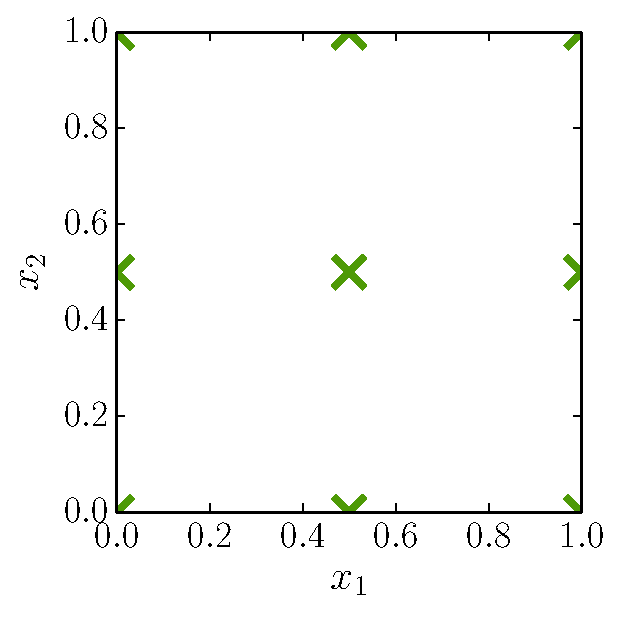
\includegraphics[height=5cm]{figures/python/opt_XD}
\end{center}
however, this design is not I-optimal nor G-optimal... 
\end{frame}

%%%%%%%%%%%%%%%%%%%%%%%%%%%%%%%%%%%%%%%%%%%%%%%%%%%%%%
\begin{frame}{known covariance parameters}
We can compute numerically the optimal shrinking factor:
\vspace{2mm}
\begin{center}
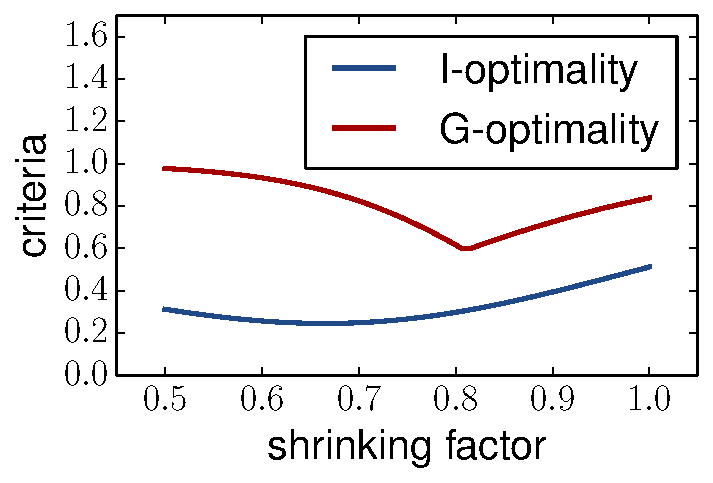
\includegraphics[height=3.9cm]{figures/python/opt_IG} \qquad
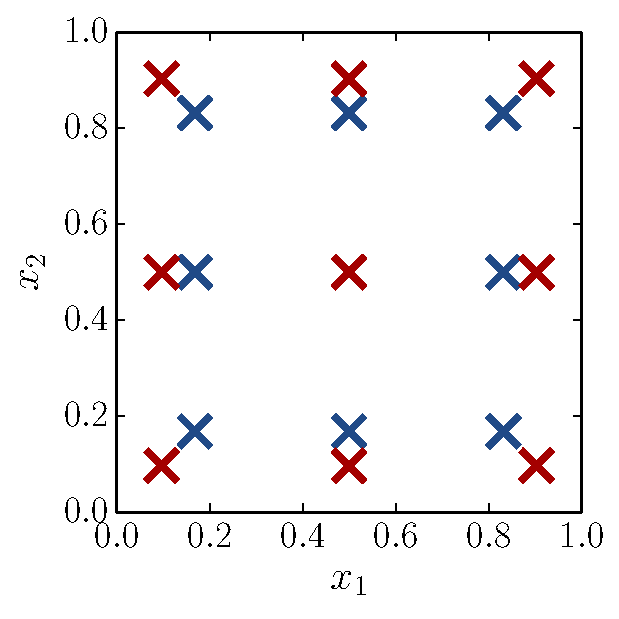
\includegraphics[height=4cm]{figures/python/opt_XIG}
\end{center}
\vspace{2mm}
$\Rightarrow$ They all give a different optimal DoE.
\end{frame}

%%%%%%%%%%%%%%%%%%%%%%%%%%%%%%%%%%%%%%%%%%%%%%%%%%%%%%
\begin{frame}{unknown covariance parameters}
What about \textbf{unknown} covariance parameter?\\
The model parameters (ie the kernel's) can be estimated using maximum likelihood. \\
\vspace{5mm}
Can we find a design that gives a good parameter estimation of the variance and lengthscale?
\begin{itemize}
	\item There is no strong theoretical results
	\item Good estimation of the variance requires the points to be far away
	\item Good estimation of the lengthscale requires the points to be close by
\end{itemize}
If the covariance structure itself is unknown, it is interesting to have in the design a large variety of inter-distances.
\end{frame}

%%%%%%%%%%%%%%%%%%%%%%%%%%%%%%%%%%%%%%%%%%%%%%%%%%%%%%
\begin{frame}{}
Small recap on optimal design for GPR
\begin{itemize}
	\item All criteria are difficult to compute
	\item The optimization problem is tricky
	\item We don't have strong theoretical results as in regression
\end{itemize}
\vspace{3mm}
Good practice:
\begin{itemize}
	\item space filling designs such as LHS
	\item Optimization inside a class of DoE
\end{itemize}
\vspace{3mm}
\structure{Remark:} IMSE is more correlated to minimax than maximin
\end{frame}

%%%%%%%%%%%%%%%%%%%%%%%%%%%%%%%%%%%%%%%%%%%%%%%%%%%%%%
%%%%%%%%%%%%%%%%%%%%%%%%%%%%%%%%%%%%%%%%%%%%%%%%%%%%%%
\section[Adaptive DoE]{Adaptive Designs}
\subsection{}

%%%%%%%%%%%%%%%%%%%%%%%%%%%%%%%%%%%%%%%%%%%%%%%%%%%%%%
\begin{frame}{}
The principle of \textbf{adaptive design} is to add the points in the design one after each other.\\
\qquad $\rightarrow$ the $n \times d$-dimensional optimisation is transformed into $n$  optimisations in $d$ dimensions.
\begin{block}{This is still expensive}
One new model has to be built for each candidate point. Furthermore, for each candidate model:
	\begin{itemize}
		\item I-optimality requires to compute a high dimensional integral
		\item G-optimality requires to optimize the variance
	\end{itemize}
\end{block}
\end{frame}

%%%%%%%%%%%%%%%%%%%%%%%%%%%%%%%%%%%%%%%%%%%%%%%%%%%%%%
\begin{frame}{}
An approximation that is not computationaly expensive is to add the new point where the model variance is maximum:
\begin{block}{Algorithm}
	\begin{itemize}
		\item[1] Build an initial DoE X with k points
		\item[2] While $i < n-k$
		\item[3] \qquad find $x^* = \mathrm{argmax}(c(x,x))$
		\item[4] \qquad add  $x^*$ to the design and recompute $c(x,x)$
	\end{itemize}
\end{block}
\end{frame}

%%%%%%%%%%%%%%%%%%%%%%%%%%%%%%%%%%%%%%%%%%%%%%%%%%%%%%
\begin{frame}{}
\vspace{5mm}
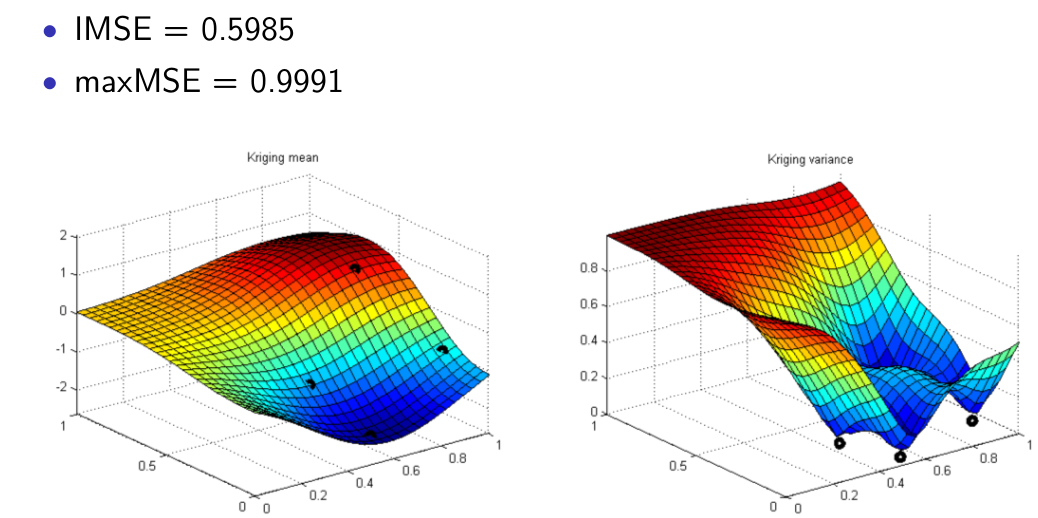
\includegraphics[width=\textwidth]{figures/adaptative1}\\
\vfill
source: Lecture from V. Picheny at Mines St-Etienne
\end{frame}

%%%%%%%%%%%%%%%%%%%%%%%%%%%%%%%%%%%%%%%%%%%%%%%%%%%%%%
\begin{frame}{}
\vspace{5mm}
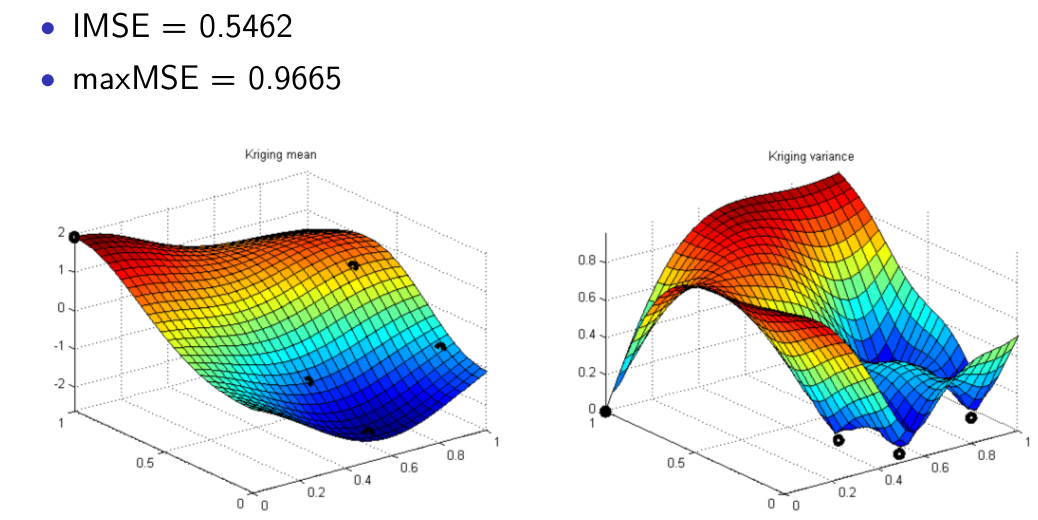
\includegraphics[width=\textwidth]{figures/adaptative2}\\
\vfill
source: Lecture from V. Picheny at Mines St-Etienne
\end{frame}

%%%%%%%%%%%%%%%%%%%%%%%%%%%%%%%%%%%%%%%%%%%%%%%%%%%%%%
\begin{frame}{}
\vspace{5mm}
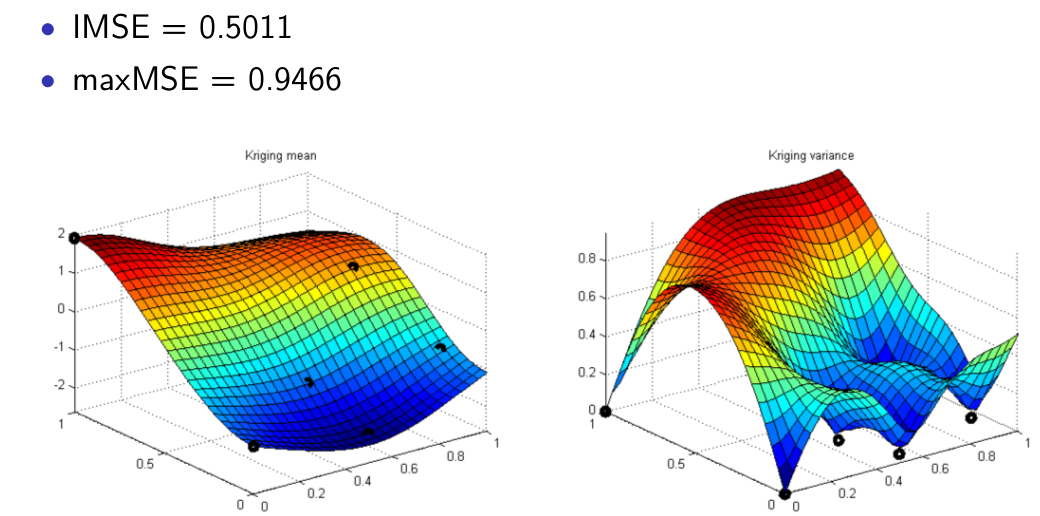
\includegraphics[width=\textwidth]{figures/adaptative3}\\
\vfill
source: Lecture from V. Picheny at Mines St-Etienne
\end{frame}

%%%%%%%%%%%%%%%%%%%%%%%%%%%%%%%%%%%%%%%%%%%%%%%%%%%%%%
\begin{frame}{}
\vspace{5mm}
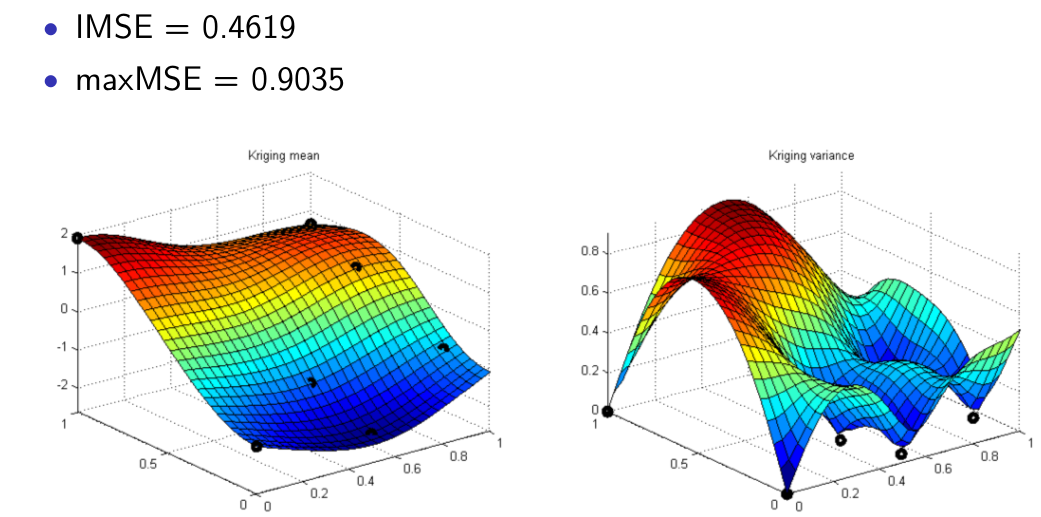
\includegraphics[width=\textwidth]{figures/adaptative4}\\
\vfill
source: Lecture from V. Picheny at Mines St-Etienne
\end{frame}

%%%%%%%%%%%%%%%%%%%%%%%%%%%%%%%%%%%%%%%%%%%%%%%%%%%%%%
\begin{frame}{}
\vspace{5mm}
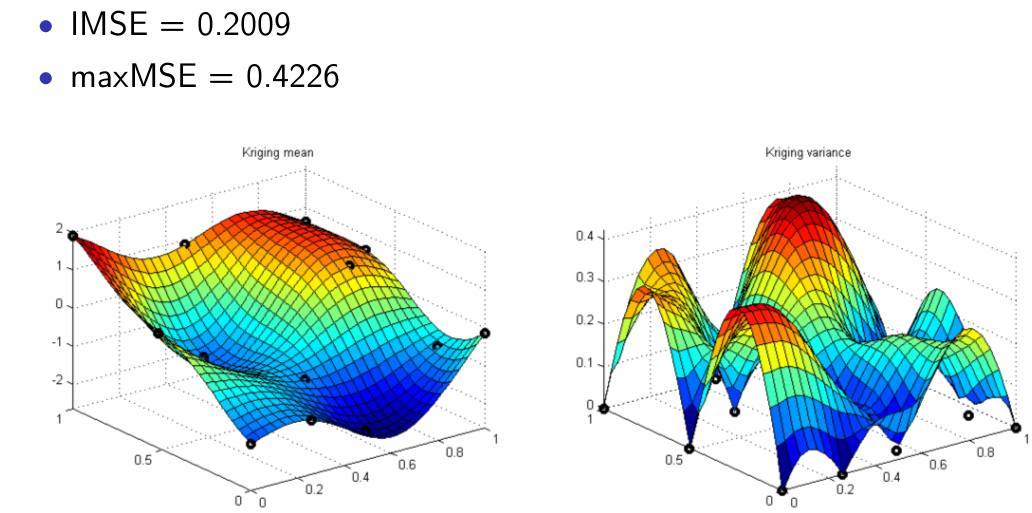
\includegraphics[width=\textwidth]{figures/adaptative6}\\
\vfill
source: Lecture from V. Picheny at Mines St-Etienne
\end{frame}

%%%%%%%%%%%%%%%%%%%%%%%%%%%%%%%%%%%%%%%%%%%%%%%%%%%%%%
\begin{frame}{}
We end-up with the following design:
\begin{columns}[c]
\column{6cm}
\begin{center}
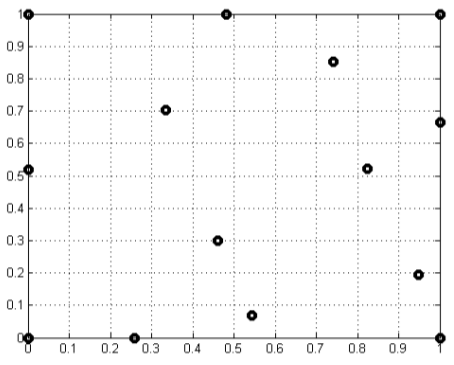
\includegraphics[height=5cm]{figures/adaptativefinal}
\end{center}
\column{5cm}
It has:
\begin{itemize}
	\item[+] Good space filling properties
	\item[$-$] Too much points on the boundaries
\end{itemize}
\end{columns}
\end{frame}

%%%%%%%%%%%%%%%%%%%%%%%%%%%%%%%%%%%%%%%%%%%%%%%%%%%%%%
%%%%%%%%%%%%%%%%%%%%%%%%%%%%%%%%%%%%%%%%%%%%%%%%%%%%%%
\section[Concl.]{Conclusion}
\subsection{}

%%%%%%%%%%%%%%%%%%%%%%%%%%%%%%%%%%%%%%%%%%%%%%%%%%%%%%
\begin{frame}{}
\begin{block}{Design of Experiments Principles}
	\begin{itemize}
		\item Control of data generation
		\item Thinking the experiments choices 
	\end{itemize}
\end{block}
\vspace{3mm}
\begin{block}{Objectives}
	\begin{itemize}
		\item Measure the influence of the variables 
		\item Get accurate models
		\item Get a good inference for the models
	\end{itemize}
\end{block}
\end{frame}

%%%%%%%%%%%%%%%%%%%%%%%%%%%%%%%%%%%%%%%%%%%%%%%%%%%%%%
\begin{frame}{Measure variables influence}
The influence of a variable can be estimated by its LR coefficient \\ \vspace{3mm}
\textbf{additive models:}
\vspace{1mm}
The number of points depends on the complexity of the univariate effects (linear quadratic, ...)
	\begin{itemize}
		\item star shaped designs
		\item one at a time designs
	\end{itemize}
\vspace{2mm}
\textbf{Models with interaction}
\vspace{1mm}
	\begin{itemize}
		\item Factorial designs
	\end{itemize}
\end{frame}


%%%%%%%%%%%%%%%%%%%%%%%%%%%%%%%%%%%%%%%%%%%%%%%%%%%%%%
\begin{frame}{Designs without model assumption}
Designs without model assumption $\rightarrow$ Space filling designs\\ \vspace{3mm}
\textbf{Various designs have been introduced} \vspace{1mm}
	\begin{itemize}
		\item Latin Hypercubes
		\item Low discrepancy sequences
		\item Centroidal voronoi tesselations 
	\end{itemize}
\vspace{3mm}
\textbf{Various criteria} \vspace{1mm}
	\begin{itemize}
		\item Quality of projection
		\item Discrepancy
		\item maximin
		\item minimax
	\end{itemize}
\end{frame}

%%%%%%%%%%%%%%%%%%%%%%%%%%%%%%%%%%%%%%%%%%%%%%%%%%%%%%
\begin{frame}{Designs with model assumption}
When the form of the model is known, we can define various optimality criteria\\ \vspace{3mm}
\textbf{Best model estimation}
\begin{itemize}
	\item D-optimality
	\item A-optimality
	\item E-optimality
\end{itemize}
\vspace{3mm}
\textbf{lowest prediction error}
\begin{itemize}
	\item G-optimality
	\item I-optimality
\end{itemize}
\vspace{3mm}
For linear regression we have some interesting results... \\
For GPR, it's much more tricky!
\end{frame}

%%%%%%%%%%%%%%%%%%%%%%%%%%%%%%%%%%%%%%%%%%%%%%%%%%%%%%
\begin{frame}{Designs optimization}
In general, optimizing DoE is difficult:
\begin{itemize}
	\item large number of variables: $n \times d$
	\item computationally expensive criteria
\end{itemize}
\vspace{3mm}
\textbf{Alternatives are:}
	\begin{itemize}
		\item Optimizing in a given class of DoE (LHD)
		\item Adaptive designs
		\item E-optimality
	\end{itemize}
\end{frame}

%Ideas : radar, DoE for additive kriging

%%%%%%%%%%%%%%%%%%%%%%%%%%%%%%%%%%%%%%%%%%%%%%%%%%%%%%%%%%%%%%%%%%%%%%%%%%%%%%%
%%%%%%%%%%%%%%%%%%%%%%%%%%%%%%%%%%%%%%%%%%%%%%%%%%%%%%%%%%%%%%%%%%%%%%%%%%%%%%%
%%%%%%%%%%%%%%%%%%%%%%%%%%%%%%%%%%%%%%%%%%%%%%%%%%%%%%%%%%%%%%%%%%%%%%%%%%%%%%%
%%%%%%%%%%%%%%%%%%%%%%%%%%%%%%%%%%%%%%%%%%%%%%%%%%%%%%%%%%%%%%%%%%%%%%%%%%%%%%%
\end{document}

###
%%%%%%%%%%%%%%%%%%%%%%%%%%%%%%%%%%%%%%%%%%%%%%%%%%%%%%
\begin{frame}{}

\end{frame}

###
\structure{}

###
\begin{center}
  \begin{tabular}{|c|cc|}

  \end{tabular}
\end{center}

###
\begin{block}{}

\end{block}

###
\begin{center}
\includegraphics[height=5cm]{figures/}
\end{center}

###
\begin{columns}[c]
\column{5cm}

\column{5cm}

\end{columns}
